
%-----------------------------------------------------------------------------
% PACKAGES AND OTHER DOCUMENT CONFIGURATIONS
%-----------------------------------------------------------------------------

\documentclass[11pt]{article}
\usepackage[margin=1in]{geometry}
\usepackage{amsmath, amsfonts}
\usepackage{enumerate}
\usepackage{graphicx}
\graphicspath{ {./images/} }
\usepackage{titling}
\usepackage{url}
\usepackage{xfrac}
\usepackage{fancyhdr}
\usepackage{geometry}
\usepackage{graphicx}
\usepackage{natbib}
\usepackage{amsmath}
\usepackage{amssymb}
\usepackage{amsthm}
\usepackage{paralist}
\usepackage{epstopdf}
\usepackage{tabularx}
\usepackage{longtable}
\usepackage{multirow}
\usepackage{multicol}
\usepackage[colorlinks=true,urlcolor=blue]{hyperref}
\usepackage{fancyvrb}
\usepackage{algorithm}
\usepackage{algorithmic}
\usepackage{float}
\usepackage{paralist}
\usepackage[svgname]{xcolor}
\usepackage{enumerate}
\usepackage{array}
\usepackage{times}
\usepackage{url}
\usepackage{fancyhdr}
\usepackage{comment}
\usepackage{environ}
\usepackage{times}
\usepackage{textcomp}
\usepackage{caption}
\usepackage[colorlinks=true,urlcolor=blue]{hyperref}
\usepackage{parskip} % For NIPS style paragraphs.
\usepackage[compact]{titlesec} % Less whitespace around titles
\usepackage[inline]{enumitem} % For inline enumerate* and itemize*
\usepackage{datetime}
\usepackage{comment}
% \usepackage{minted}
\usepackage{lastpage}
\usepackage{color}
\usepackage{xcolor}
\usepackage{tikz}
\usetikzlibrary{shapes,decorations}
\usepackage{framed}
\usepackage{booktabs}
\usepackage{cprotect}
\usepackage{fancyvrb}
\usepackage{xcolor}
\usepackage{verbatimbox}
\usepackage[final]{listings}



\usepackage{xcolor}
\usepackage{verbatimbox}
\usepackage[many]{tcolorbox}
\newcommand{\blackcircle}{\tikz\draw[black,fill=black] (0,0) circle (1ex);}
\renewcommand{\circle}{\tikz\draw[black] (0,0) circle (1ex);}
\newtcolorbox[]{solution}[1][]{%
    breakable,
    enhanced,
    colback=white,
    title=Solution,
    #1
}
\usepackage{cancel}

%%%%%%%%%%%%%%%%%%%%%%%%%%%%%%%%%%%%%%%%%%%
% Better numbering                        %
%%%%%%%%%%%%%%%%%%%%%%%%%%%%%%%%%%%%%%%%%%%

\numberwithin{equation}{section} % Number equations within sections (i.e. 1.1, 1.2, 2.1, 2.2 instead of 1, 2, 3, 4)
\numberwithin{figure}{section} % Number figures within sections (i.e. 1.1, 1.2, 2.1, 2.2 instead of 1, 2, 3, 4)
\numberwithin{table}{section} % Number tables within sections (i.e. 1.1, 1.2, 2.1, 2.2 instead of 1, 2, 3, 4)

%%%%%%%%%%%%%%%%%%%%%%%%%%%%%%%%%%%%%%%%%%
% Custom commands                        %
%%%%%%%%%%%%%%%%%%%%%%%%%%%%%%%%%%%%%%%%%%

\def\x{\mathbf x}
\def\y{\mathbf y}
\def\w{\mathbf w}
\def\v{\mathbf v}
\def\E{\mathbb E}
\def\V{\mathbb V}


% mathcal
\newcommand{\Ac}{\mathcal{A}}
\newcommand{\Bc}{\mathcal{B}}
\newcommand{\Cc}{\mathcal{C}}
\newcommand{\Dc}{\mathcal{D}}
\newcommand{\Ec}{\mathcal{E}}
\newcommand{\Fc}{\mathcal{F}}
\newcommand{\Gc}{\mathcal{G}}
\newcommand{\Hc}{\mathcal{H}}
\newcommand{\Ic}{\mathcal{I}}
\newcommand{\Jc}{\mathcal{J}}
\newcommand{\Kc}{\mathcal{K}}
\newcommand{\Lc}{\mathcal{L}}
\newcommand{\Mc}{\mathcal{M}}
\newcommand{\Nc}{\mathcal{N}}
\newcommand{\Oc}{\mathcal{O}}
\newcommand{\Pc}{\mathcal{P}}
\newcommand{\Qc}{\mathcal{Q}}
\newcommand{\Rc}{\mathcal{R}}
\newcommand{\Sc}{\mathcal{S}}
\newcommand{\Tc}{\mathcal{T}}
\newcommand{\Uc}{\mathcal{U}}
\newcommand{\Vc}{\mathcal{V}}
\newcommand{\Wc}{\mathcal{W}}
\newcommand{\Xc}{\mathcal{X}}
\newcommand{\Yc}{\mathcal{Y}}
\newcommand{\Zc}{\mathcal{Z}}

% mathbb
\newcommand{\Ab}{\mathbb{A}}
\newcommand{\Bb}{\mathbb{B}}
\newcommand{\Cb}{\mathbb{C}}
\newcommand{\Db}{\mathbb{D}}
\newcommand{\Eb}{\mathbb{E}}
\newcommand{\Fb}{\mathbb{F}}
\newcommand{\Gb}{\mathbb{G}}
\newcommand{\Hb}{\mathbb{H}}
\newcommand{\Ib}{\mathbb{I}}
\newcommand{\Jb}{\mathbb{J}}
\newcommand{\Kb}{\mathbb{K}}
\newcommand{\Lb}{\mathbb{L}}
\newcommand{\Mb}{\mathbb{M}}
\newcommand{\Nb}{\mathbb{N}}
\newcommand{\Ob}{\mathbb{O}}
\newcommand{\Pb}{\mathbb{P}}
\newcommand{\Qb}{\mathbb{Q}}
\newcommand{\Rb}{\mathbb{R}}
\newcommand{\Sb}{\mathbb{S}}
\newcommand{\Tb}{\mathbb{T}}
\newcommand{\Ub}{\mathbb{U}}
\newcommand{\Vb}{\mathbb{V}}
\newcommand{\Wb}{\mathbb{W}}
\newcommand{\Xb}{\mathbb{X}}
\newcommand{\Yb}{\mathbb{Y}}
\newcommand{\Zb}{\mathbb{Z}}

% mathbf lowercase
\newcommand{\av}{\mathbf{a}}
\newcommand{\bv}{\mathbf{b}}
\newcommand{\cv}{\mathbf{c}}
\newcommand{\dv}{\mathbf{d}}
\newcommand{\ev}{\mathbf{e}}
\newcommand{\fv}{\mathbf{f}}
\newcommand{\gv}{\mathbf{g}}
\newcommand{\hv}{\mathbf{h}}
\newcommand{\iv}{\mathbf{i}}
\newcommand{\jv}{\mathbf{j}}
\newcommand{\kv}{\mathbf{k}}
\newcommand{\lv}{\mathbf{l}}
\newcommand{\mv}{\mathbf{m}}
\newcommand{\nv}{\mathbf{n}}
\newcommand{\ov}{\mathbf{o}}
\newcommand{\pv}{\mathbf{p}}
\newcommand{\qv}{\mathbf{q}}
\newcommand{\rv}{\mathbf{r}}
\newcommand{\sv}{\mathbf{s}}
\newcommand{\tv}{\mathbf{t}}
\newcommand{\uv}{\mathbf{u}}
\newcommand{\vv}{\mathbf{v}}
\newcommand{\wv}{\mathbf{w}}
\newcommand{\xv}{\mathbf{x}}
\newcommand{\yv}{\mathbf{y}}
\newcommand{\zv}{\mathbf{z}}

% mathbf uppercase
\newcommand{\Av}{\mathbf{A}}
\newcommand{\Bv}{\mathbf{B}}
\newcommand{\Cv}{\mathbf{C}}
\newcommand{\Dv}{\mathbf{D}}
\newcommand{\Ev}{\mathbf{E}}
\newcommand{\Fv}{\mathbf{F}}
\newcommand{\Gv}{\mathbf{G}}
\newcommand{\Hv}{\mathbf{H}}
\newcommand{\Iv}{\mathbf{I}}
\newcommand{\Jv}{\mathbf{J}}
\newcommand{\Kv}{\mathbf{K}}
\newcommand{\Lv}{\mathbf{L}}
\newcommand{\Mv}{\mathbf{M}}
\newcommand{\Nv}{\mathbf{N}}
\newcommand{\Ov}{\mathbf{O}}
\newcommand{\Pv}{\mathbf{P}}
\newcommand{\Qv}{\mathbf{Q}}
\newcommand{\Rv}{\mathbf{R}}
\newcommand{\Sv}{\mathbf{S}}
\newcommand{\Tv}{\mathbf{T}}
\newcommand{\Uv}{\mathbf{U}}
\newcommand{\Vv}{\mathbf{V}}
\newcommand{\Wv}{\mathbf{W}}
\newcommand{\Xv}{\mathbf{X}}
\newcommand{\Yv}{\mathbf{Y}}
\newcommand{\Zv}{\mathbf{Z}}

% bold greek lowercase
\newcommand{\alphav     }{\boldsymbol \alpha     }
\newcommand{\betav      }{\boldsymbol \beta      }
\newcommand{\gammav     }{\boldsymbol \gamma     }
\newcommand{\deltav     }{\boldsymbol \delta     }
\newcommand{\epsilonv   }{\boldsymbol \epsilon   }
\newcommand{\varepsilonv}{\boldsymbol \varepsilon}
\newcommand{\zetav      }{\boldsymbol \zeta      }
\newcommand{\etav       }{\boldsymbol \eta       }
\newcommand{\thetav     }{\boldsymbol \theta     }
\newcommand{\varthetav  }{\boldsymbol \vartheta  }
\newcommand{\iotav      }{\boldsymbol \iota      }
\newcommand{\kappav     }{\boldsymbol \kappa     }
\newcommand{\varkappav  }{\boldsymbol \varkappa  }
\newcommand{\lambdav    }{\boldsymbol \lambda    }
\newcommand{\muv        }{\boldsymbol \mu        }
\newcommand{\nuv        }{\boldsymbol \nu        }
\newcommand{\xiv        }{\boldsymbol \xi        }
\newcommand{\omicronv   }{\boldsymbol \omicron   }
\newcommand{\piv        }{\boldsymbol \pi        }
\newcommand{\varpiv     }{\boldsymbol \varpi     }
\newcommand{\rhov       }{\boldsymbol \rho       }
\newcommand{\varrhov    }{\boldsymbol \varrho    }
\newcommand{\sigmav     }{\boldsymbol \sigma     }
\newcommand{\varsigmav  }{\boldsymbol \varsigma  }
\newcommand{\tauv       }{\boldsymbol \tau       }
\newcommand{\upsilonv   }{\boldsymbol \upsilon   }
\newcommand{\phiv       }{\boldsymbol \phi       }
\newcommand{\varphiv    }{\boldsymbol \varphi    }
\newcommand{\chiv       }{\boldsymbol \chi       }
\newcommand{\psiv       }{\boldsymbol \psi       }
\newcommand{\omegav     }{\boldsymbol \omega     }

% bold greek uppercase
\newcommand{\Gammav     }{\boldsymbol \Gamma     }
\newcommand{\Deltav     }{\boldsymbol \Delta     }
\newcommand{\Thetav     }{\boldsymbol \Theta     }
\newcommand{\Lambdav    }{\boldsymbol \Lambda    }
\newcommand{\Xiv        }{\boldsymbol \Xi        }
\newcommand{\Piv        }{\boldsymbol \Pi        }
\newcommand{\Sigmav     }{\boldsymbol \Sigma     }
\newcommand{\Upsilonv   }{\boldsymbol \Upsilon   }
\newcommand{\Phiv       }{\boldsymbol \Phi       }
\newcommand{\Psiv       }{\boldsymbol \Psi       }
\newcommand{\Omegav     }{\boldsymbol \Omega     }


%%%%%%%%%%%%%%%%%%%%%%%%%%%%%%%%%%%%%%%%%%%
% Code highlighting with listings         %
%%%%%%%%%%%%%%%%%%%%%%%%%%%%%%%%%%%%%%%%%%%

\definecolor{bluekeywords}{rgb}{0.13,0.13,1}
\definecolor{greencomments}{rgb}{0,0.5,0}
\definecolor{redstrings}{rgb}{0.9,0,0}
\definecolor{light-gray}{gray}{0.95}

\newcommand{\MYhref}[3][blue]{\href{#2}{\color{#1}{#3}}}%

\definecolor{dkgreen}{rgb}{0,0.6,0}
\definecolor{gray}{rgb}{0.5,0.5,0.5}
\definecolor{mauve}{rgb}{0.58,0,0.82}

\lstdefinelanguage{Shell}{
  keywords={tar, cd, make},
  %keywordstyle=\color{bluekeywords}\bfseries,
  alsoletter={+},
  ndkeywords={python, py, javac, java, gcc, c, g++, cpp, .txt, octave, m, .tar},
  %ndkeywordstyle=\color{bluekeywords}\bfseries,
  identifierstyle=\color{black},
  sensitive=false,
  comment=[l]{//},
  morecomment=[s]{/*}{*/},
  commentstyle=\color{purple}\ttfamily,
  stringstyle=\color{red}\ttfamily,
  morestring=[b]',
  morestring=[b]",
  backgroundcolor = \color{light-gray}
}

\lstset{columns=fixed, basicstyle=\ttfamily,
    backgroundcolor=\color{light-gray},xleftmargin=0.5cm,frame=tlbr,framesep=4pt,framerule=0pt}


%%%%%%%%%%%%%%%%%%%%%%%%%%%%%%%%%%%%%%%%%%%
% Rotated Column Headers                  %
%%%%%%%%%%%%%%%%%%%%%%%%%%%%%%%%%%%%%%%%%%%
\usepackage{adjustbox}
\usepackage{array}

%https://tex.stackexchange.com/questions/32683/rotated-column-titles-in-tabular

\newcolumntype{R}[2]{%
    >{\adjustbox{angle=#1,lap=\width-(#2)}\bgroup}%
    l%
    <{\egroup}%
}
\newcommand*\rot{\multicolumn{1}{R{45}{1em}}}% no optional argument here, please!

%%%%%%%%%%%%%%%%%%%%%%%%%%%%%%%%%%%%%%%%%%%
% Custom box for highlights               %
%%%%%%%%%%%%%%%%%%%%%%%%%%%%%%%%%%%%%%%%%%%

% Define box and box title style
\tikzstyle{mybox} = [fill=blue!10, very thick,
    rectangle, rounded corners, inner sep=1em, inner ysep=1em]

% \newcommand{\notebox}[1]{
% \begin{tikzpicture}
% \node [mybox] (box){%
%     \begin{minipage}{\textwidth}
%     #1
%     \end{minipage}
% };
% \end{tikzpicture}%
% }

\NewEnviron{notebox}{
\begin{tikzpicture}
\node [mybox] (box){
    \begin{minipage}{\textwidth}
        \BODY
    \end{minipage}
};
\end{tikzpicture}
}

%%%%%%%%%%%%%%%%%%%%%%%%%%%%%%%%%%%%%%%%%%%
% Commands showing / hiding solutions     %
%%%%%%%%%%%%%%%%%%%%%%%%%%%%%%%%%%%%%%%%%%%



%% To HIDE SOLUTIONS (to post at the website for students), set this value to 0: \def\issoln{0}
% \def\issoln{0}
\def\issoln{0}
% Some commands to allow solutions to be embedded in the assignment file.
\ifcsname issoln\endcsname \else \def\issoln{1} \fi
% Default to an empty solutions environ.
\NewEnviron{soln}{}{}
\if\issoln 1
% Otherwise, include solutions as below.
 \RenewEnviron{soln}{
     \leavevmode\color{red}\ignorespaces
     \textbf{Solution} \BODY
 }{}
 \fi

%%%%%%%%%%%%%%%%%%%%%%%%%%%%%%%%%%%%%%%%%%%
% Commands for customizing the assignment %
%%%%%%%%%%%%%%%%%%%%%%%%%%%%%%%%%%%%%%%%%%%

\newcommand{\courseName}{10-601 Introduction to Machine Learning (Fall 2019)}
\newcommand{\hwName}{Homework 4: Logistic Regression}
\newcommand{\outDate}{Wed, Sep 25, 2019}
\newcommand{\dueDate}{Fri, Oct 11, 2019 11:59 PM}

\pagestyle{fancyplain}
\lhead{\fancyplain{}{\hwName}}
\rhead{\fancyplain{}{\courseName}}
\cfoot{\thepage}

\title{\textsc{\hwName}} % Title


\author{\courseName\\
  Carnegie Mellon University \\
\url{piazza.com/cmu/fall2019/1030110601} \\
OUT: \outDate{} \thanks{Compiled on \today{} at \currenttime{}} \\
DUE: \dueDate{} \\ 
TAs: Max Le, Bharath Prabhu, Manini Amin, and Anupma Shara}

\date{}

%%%%%%%%%%%%%%%%%%%%%%%%%%%%%%%%%%%%%%%%%%%%%%%%%
% Useful commands for typesetting the questions %
%%%%%%%%%%%%%%%%%%%%%%%%%%%%%%%%%%%%%%%%%%%%%%%%%

\newcommand \expect {\mathbb{E}}
\newcommand \mle [1]{{\hat #1}^{\rm MLE}}
\newcommand \map [1]{{\hat #1}^{\rm MAP}}
\newcommand \argmax {\operatorname*{argmax}}
\newcommand \argmin {\operatorname*{argmin}}
\newcommand \code [1]{{\tt #1}}
\newcommand \datacount [1]{\#\{#1\}}
\newcommand \ind [1]{\mathbb{I}\{#1\}}

%%%%%%%%%%%%%%%%%%%%%%%%%%
% Document configuration %
%%%%%%%%%%%%%%%%%%%%%%%%%%

% Don't display a date in the title and remove the white space
\predate{}
\postdate{}
\date{}

% Don't display an author and remove the white spacez
%\preauthor{}
%\postauthor{}

%%%%%%%%%%%%%%%%%%
% Begin Document %
%%%%%%%%%%%%%%%%%% 

\begin{document}

\maketitle

\begin{notebox}
\paragraph{Summary} In this assignment, you will build a sentiment polarity analyzer, which will be capable of analyzing the overall sentiment polarity (positive or negative) . In Section  \ref{sec:written} you will warm up by deriving stochastic gradient descent updates for binary and multinomial logistic regression. Then in Section \ref{programming} you will implement a binary logistic regression model as the core of your natural language processing system.
\end{notebox}

\section*{START HERE: Instructions}
\begin{itemize}

\item \textbf{Collaboration Policy}: Collaboration on solving the homework is allowed, after you have thought about the problems on your own. It is also OK to get clarification (but not solutions) from books or online resources, again after you have thought about the problems on your own. There are two requirements: first, cite your collaborators fully and completely (e.g., ``Jane explained to me what is asked in Question 3.4''). Second, write your solution {\em independently}: close the book and all of your notes, and send collaborators out of the room, so that the solution comes from you only.  See the collaboration policy on the website for more information: \url{http://www.cs.cmu.edu/~mgormley/courses/10601/about.html#7-academic-integrity-policies}
\item\textbf{Late Submission Policy:} See the late submission policy
  here:
  \url{http://www.cs.cmu.edu/~mgormley/courses/10601/about.html#late-homework-policy}

\item\textbf{Submitting your work:} You will use Gradescope to submit
  answers to all questions, and Autolab to submit your code. Please
  follow instructions at the end of this PDF to correctly submit all your code to Autolab.

  \begin{itemize}
    
  % COMMENT IF NOT USING CANVAS
\begin{comment}
  \item \textbf{Canvas:} Canvas (\url{https://canvas.cmu.edu}) will be
    used for quiz-style problems (e.g. multiple choice, true / false,
    numerical answers). Grading is done automatically.
    %
    You may only \textbf{submit once} on canvas, so be sure of your
    answers before you submit. However, canvas allows you to work on
    your answers and then close out of the page and it will save your
    progress.  You will not be granted additional submissions, so
    please be confident of your solutions when you are submitting your
    assignment.
    %
    {\color{red} The above is true for future assignments, but this one
    allows {\bf unlimited submissions}.}
\end{comment}
    
  % COMMENT IF NOT USING GRADESCOPE
   \item \textbf{Gradescope:} For written problems such as derivations,
       proofs, or plots we will be using Gradescope
       (\url{https://gradescope.com/}). Submissions can be handwritten, but
       should be labeled and clearly legible. If your writing is not
       legible, you will not be awarded marks. Alternatively, submissions
       can be written in LaTeX. Upon submission, label each question
       using the template provided. Regrade requests can be made, however
       this gives the TA the opportunity to regrade your entire paper,
       meaning if additional mistakes are found then points will be
       deducted.
       %   
       Each derivation/proof should be  completed on a separate page.

  %   COMMENT IF NOT USING AUTOLAB
  \item \textbf{Autolab:} You will submit your code for programming
    questions on the homework to Autolab
    (\url{https://autolab.andrew.cmu.edu/}). After uploading your code,
    our grading scripts will autograde your assignment by running your
    program on a virtual machine (VM). 
    %
    When you are developing, check that the
    version number of the programming language environment
    (e.g. Python 2.7.6/3.6.8, Octave 3.8.2, OpenJDK 1.8.0, g++ 4.8.5) and
    versions of permitted libraries (e.g.  \texttt{numpy} 1.11.1 and \texttt{scipy} 0.18.1) 
    match those used on Autolab.
    % 
    Octave users: Please make sure you do not use any
    Matlab-specific libraries in your code that might make it fail
    against our tests.
    %
    Python3 users: Please include a blank file called python3.txt (case-sensitive) in your tar submission. 
    %
    You have a {\bf total of 10 Autolab submissions}. Use them
    wisely. In order to not waste Autolab submissions, we recommend
    debugging your implementation on your local machine (or the linux
    servers) and making sure your code is running correctly first
    before any Autolab submission. 
    %

  \end{itemize}
  
\item\textbf{Materials:} Download from autolab the tar file ("Download
  handout"). The tar file will contain all the data that you will need in order to complete this assignment.

\end{itemize}


\begin{notebox}
\paragraph{Linear Algebra Libraries} When implementing machine learning algorithms, it is often convenient to have a linear algebra library at your disposal. In this assignment, Java users may use EJML\footnote{\url{https://ejml.org}} and C++ users Eigen\footnote{\url{http://eigen.tuxfamily.org/}}. Details below. 
%
(As usual, Python users have numpy; Octave users have built-in matrix support.)
%
\begin{description}
\item[Java] EJML is a pure Java linear algebra package with three interfaces. We strongly recommend using the SimpleMatrix interface. Autolab will use EJML version 3.3. The command line arguments above demonstrate how we will call you code. The classpath inclusion \lstinline{-cp "./lib/ejml-v0.33-libs/*:./"} will ensure that all the EJML jars are on the classpath as well as your code. 
\item[C++] Eigen is a header-only library, so there is no linking to worry about---just \lstinline{#include} whatever components you need. Autolab will use Eigen version 3.3.4. The command line arguments above demonstrate how we will call you code. The argument \lstinline{-I./lib} will include the \lstinline{lib/Eigen} subdirectory, which contains all the headers.
\end{description} 
We have included the correct versions of EJML/Eigen in the handout.tar for your convenience. Do {\bf not} include EJML or Eigen in your Autolab submission tar; the autograder will ensure that they are in place. 
\end{notebox}


\clearpage

\section{Written Questions [30 points]}
\label{sec:written}

\subsection{Perceptron and Stochastic Gradient Descent [4 points]}
\begin{enumerate}
    
    \item \textbf{[2 points]} We can view the perceptron algorithm as trying to minimize which of the following loss functions with stochastic gradient descent? Assume that we apply the notation where $x_0 = 1$. $\theta_0$ is the bias term, and $N$ is the number of data points. You may use the notation
    $$
    (x)_+ =
    \begin{cases}
    x, & \textrm{ if } x \geq 0 \\
    0, & \textrm{ otherwise}
    \end{cases}
    $$

    \textbf{Select one:}
    \begin{list}{}
        \item $\circle$ $J(\theta) = \sum_{i=1}^N -y^{(i)}\left(\theta^T \xv^{(i)}\right)$
        \item $\circle$ $J(\theta) = \sum_{i=1}^N y^{(i)}\left(\theta^T \xv^{(i)}\right)$
        \item $\blackcircle$ $J(\theta) = \sum_{i=1}^N \left(-y^{(i)}\left(\theta^T \xv^{(i)}\right)\right)_+$
        \item $\circle$ $J(\theta) = \sum_{i=1}^N \left(y^{(i)}\left(\theta^T \xv^{(i)}\right)\right)_+$
    \end{list}


    \item \textbf{[2 points]} Continuing with the above question, what is the gradient of the correct loss function when the current data we are seeing is $\left(\xv^{(i)}, y^{(i)}\right)$?

    \textbf{Select one:}
    \begin{list}{}
        \item $\blackcircle$ $\begin{cases}-y^{(i)}\xv^{(i)}, & \textrm{ if } -y^{(i)}\left(\theta\cdot \xv^{(i)}\right) \geq 0 \\
        0, & \textrm{ otherwise}.
        \end{cases}$
        \item $\circle$ $-y^{(i)}\xv^{(i)}$
        \item $\circle$ $y^{(i)}\xv^{(i)}$
        \item $\circle$ $\begin{cases}y^{(i)}\xv^{(i)}, & \textrm{ if } -y^{(i)}\left(\theta\cdot \xv^{(i)}\right) \geq 0 \\
        0, & \textrm{ otherwise}.
        \end{cases}$
    \end{list}

    
\end{enumerate}
\clearpage

\subsection{Multinomial Logistic Regression [13 points]}
Multinomial logistic regression, also known as softmax regression or multiclass logistic regression, is a generalization of binary logistic regression. In this problem setting we have a dataset:
\[
\mathcal{D} = \left\{\left(\xv^{(1)}, y^{(1)}\right), \ldots, \left(\xv^{(N)}, y^{(N)}\right)\right\} \text{ where } \xv^{(i)} \in \Rb^M, y^{(i)} \in \{1, \ldots, K\} \text{ for } i = 1, \ldots, N
\]
Here $N$ is the number of training examples, $M$ is the number of features, and $K$ is the number of possible classes, which is usually greater than two to be interesting and not equivalent to binary logistic regression.

\begin{enumerate}[label=(\alph*)]
    
    \item {\bf [2 points]} To motivate multinomial logistic regression, we will first look at a general way to extend a binary classifier to a multiclass classifier and apply it to logistic regression. Suppose we only have the resources to train $K$ \emph{binary logistic regression} classifiers where $K$ corresponds to the number of classes. Using all of the trained classifiers, what are the possible ways to determine the class for each unlabelled data point $\xv^{(*)}$
    
    \textbf{Select all that apply:}
    \begin{list}{}
        \item $\blacksquare$  Each trained classifier $h_i(\xv)$  will determine if a point $\xv$ is in class $i$ or not for $i = 1, \ldots, K$. The class that has the highest probability from the K classifiers will be the predicted label of point $\xv$ 
        \item $\square$  Each trained classifier $h_i(\xv)$  will determine if a point $\xv$ is in class $i$ or not for $i = 1, \ldots, K$. The class that has the highest 'confidence score' from the K classifiers will be the predicted label of point $\xv$, where 'confidence score' of classifier $i$ is defined as $\wv^T_i \xv + b$
        \item $\blacksquare$  Each trained classifier $h_i(\xv)$  will determine if a point $\xv$ is in class $i$ or not for $i = 1, \ldots, K$. The class that has the highest 'confidence score' from the K classifiers will be the predicted label of point $\xv$, where 'confidence score' of classifier $i$ is defined as $\frac{\wv^T_i \xv + b}{| \wv_i |}$ (the signed distance from a point to the plane defined by $\wv_i^T \xv + b = 0$)   
        \item $\square$ Each trained classifier $h_i(\xv)$  will determine if a point $\xv$ is in class $i$ or class $j$ for all possible combinations of $i$ and $j$ where $i = 1, \ldots, K$ and  $j = 1, \ldots, K$. The class label that is predicted the most number of times by the $K$ classifiers is assigned to point $\xv$
    \end{list}
    
    
    \item {\bf [1 point]} Now we would like a method to do multiclass classification without having to train more than one classifier. Multinomial logistic regression is such a method. Remember that in multinomial logistic regression, we have
    \begin{equation} \label{eq:1}
        p\left(y \mid \xv, \Thetav\right) = \frac{\exp\left(\thetav_{y} \xv \right)}{\sum_{j = 1}^K \exp\left(\thetav_{j} \xv\right)} = \text{softmax}((\Thetav \xv)_y)
    \end{equation}

    where $\Thetav$ is the parameter matrix of size $K \times (M + 1)$ and $\thetav_y$ denotes the $y$th \textbf{row} of $\Thetav$, which is the parameter vector for class $y$. Since we have folded the bias term into $\Thetav$ we now have $\xv \in \Rb^{M + 1}$. Let us represent class $C_k$ with a \emph{one-hot encoding}, specifically let $C_k \in \Rb^K$ where the $k$th entry in $C_k$ is 1, and 0 everywhere else. Let us also define a target matrix $\Tv$ of size $N \times K$, where the $i$th {\bf row} of $\Tv$ is $C_{y^{(i)}}$, where only the  $y^{(i)}$th entry is 1, and 0 else where.
    
    Write down the data conditional likelihood $ \mathcal{L}(\Thetav \mid \Tv, \Xv)$ in terms of $N$, $K$, $\Tv$ and $p\left(C_j \mid x^{(i)}, \Thetav \right)$. Please note that $\mathcal{L}(\Thetav \mid \Tv, \Xv) = p(\Tv \mid \Thetav, \Xv)$, where likelihood is a function of parameters (not probability), and it is equal in value to the label probability conditioned on data and parameters.
    
    \begin{solution}
    % If you are using the latex template, remove the empty spaces
    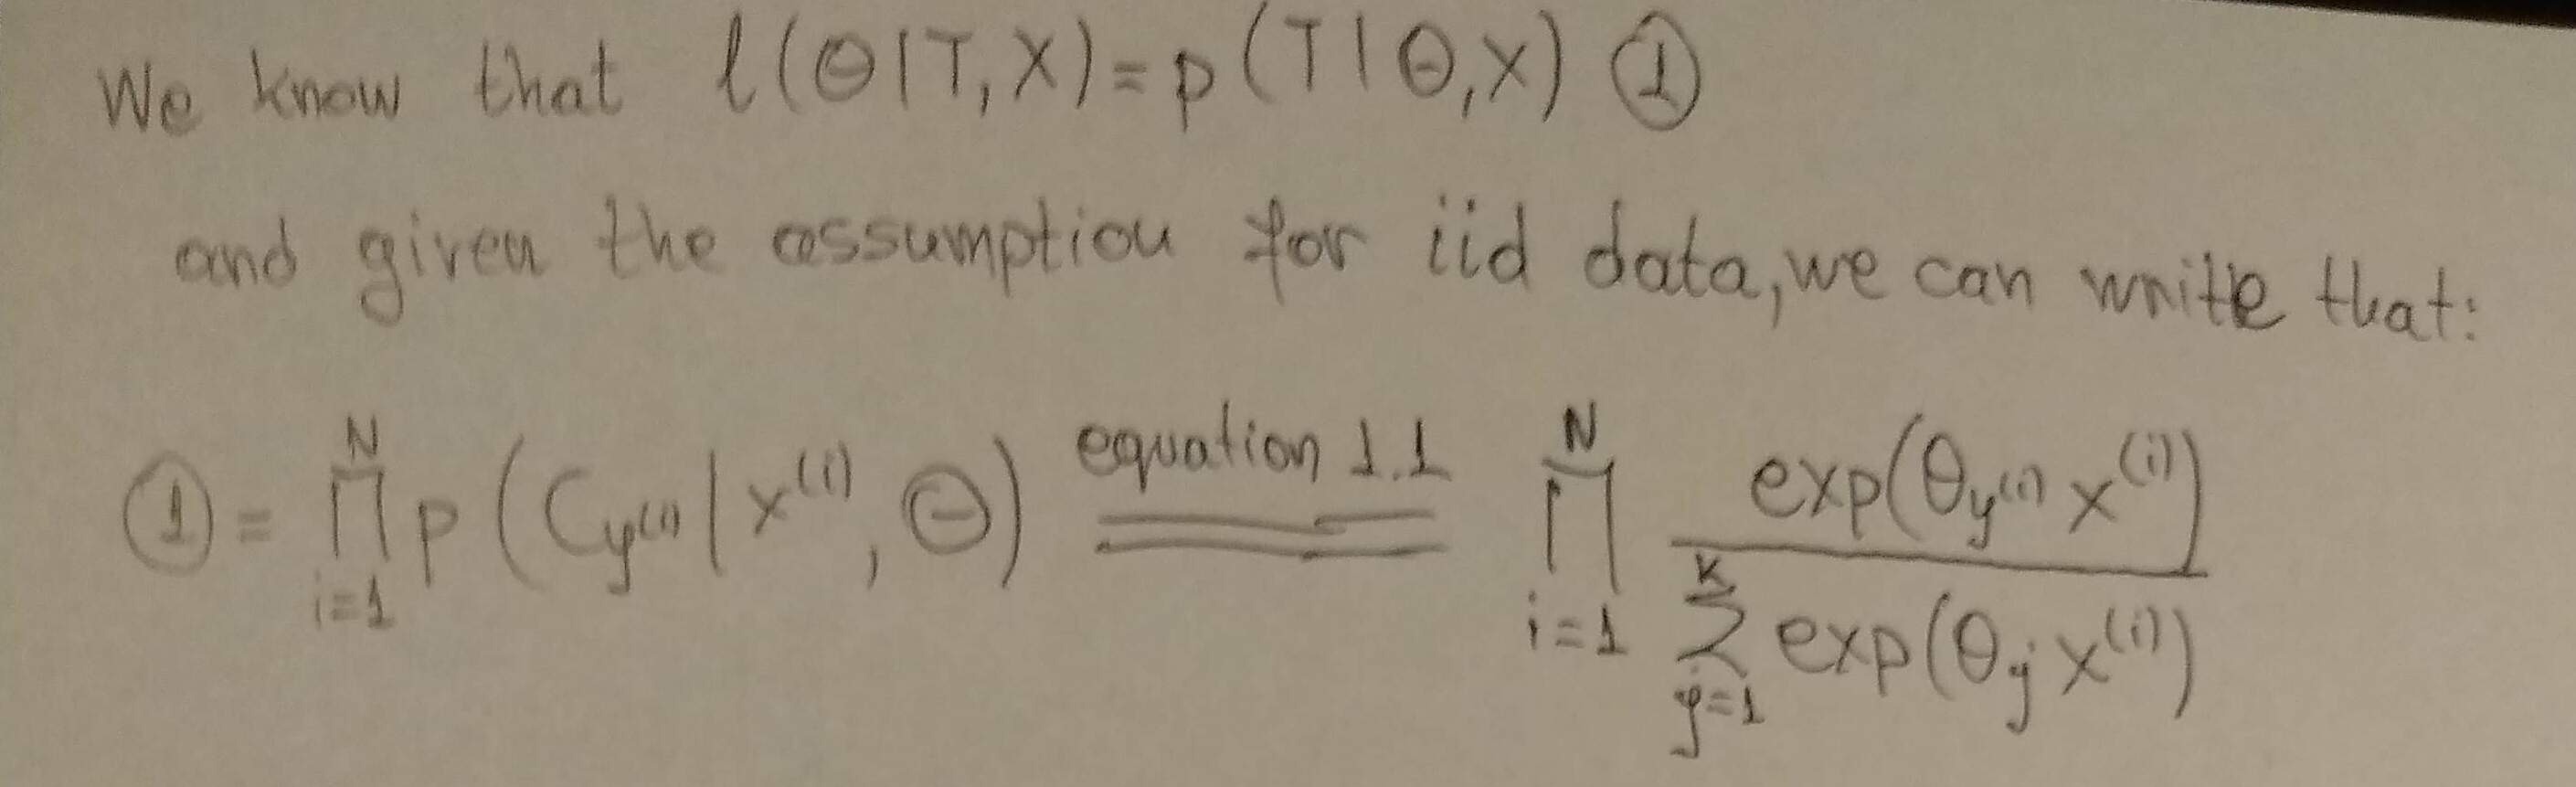
\includegraphics[scale=0.14]{pic1}
    \end{solution}
    % \clearpage
    
    
    \item {\bf [1 point]} Write down the \emph{negative} conditional log-likelihood of the data in terms of $N$, $K$, $\Tv$ and $p\left(C_j \mid x^{(i)}, \Thetav \right)$. This will be your objective function $J(\Thetav)$, also known as cross-entropy loss. To help you with the next part, write down the objective function after replacing $p\left(C_j \mid x^{(i)}, \Thetav \right)$ using equation \ref{eq:1} given in part (b). Do not include the literal term "softmax" in your answer.
    
     \begin{solution}
    % If you are using the latex template, remove the empty spaces
    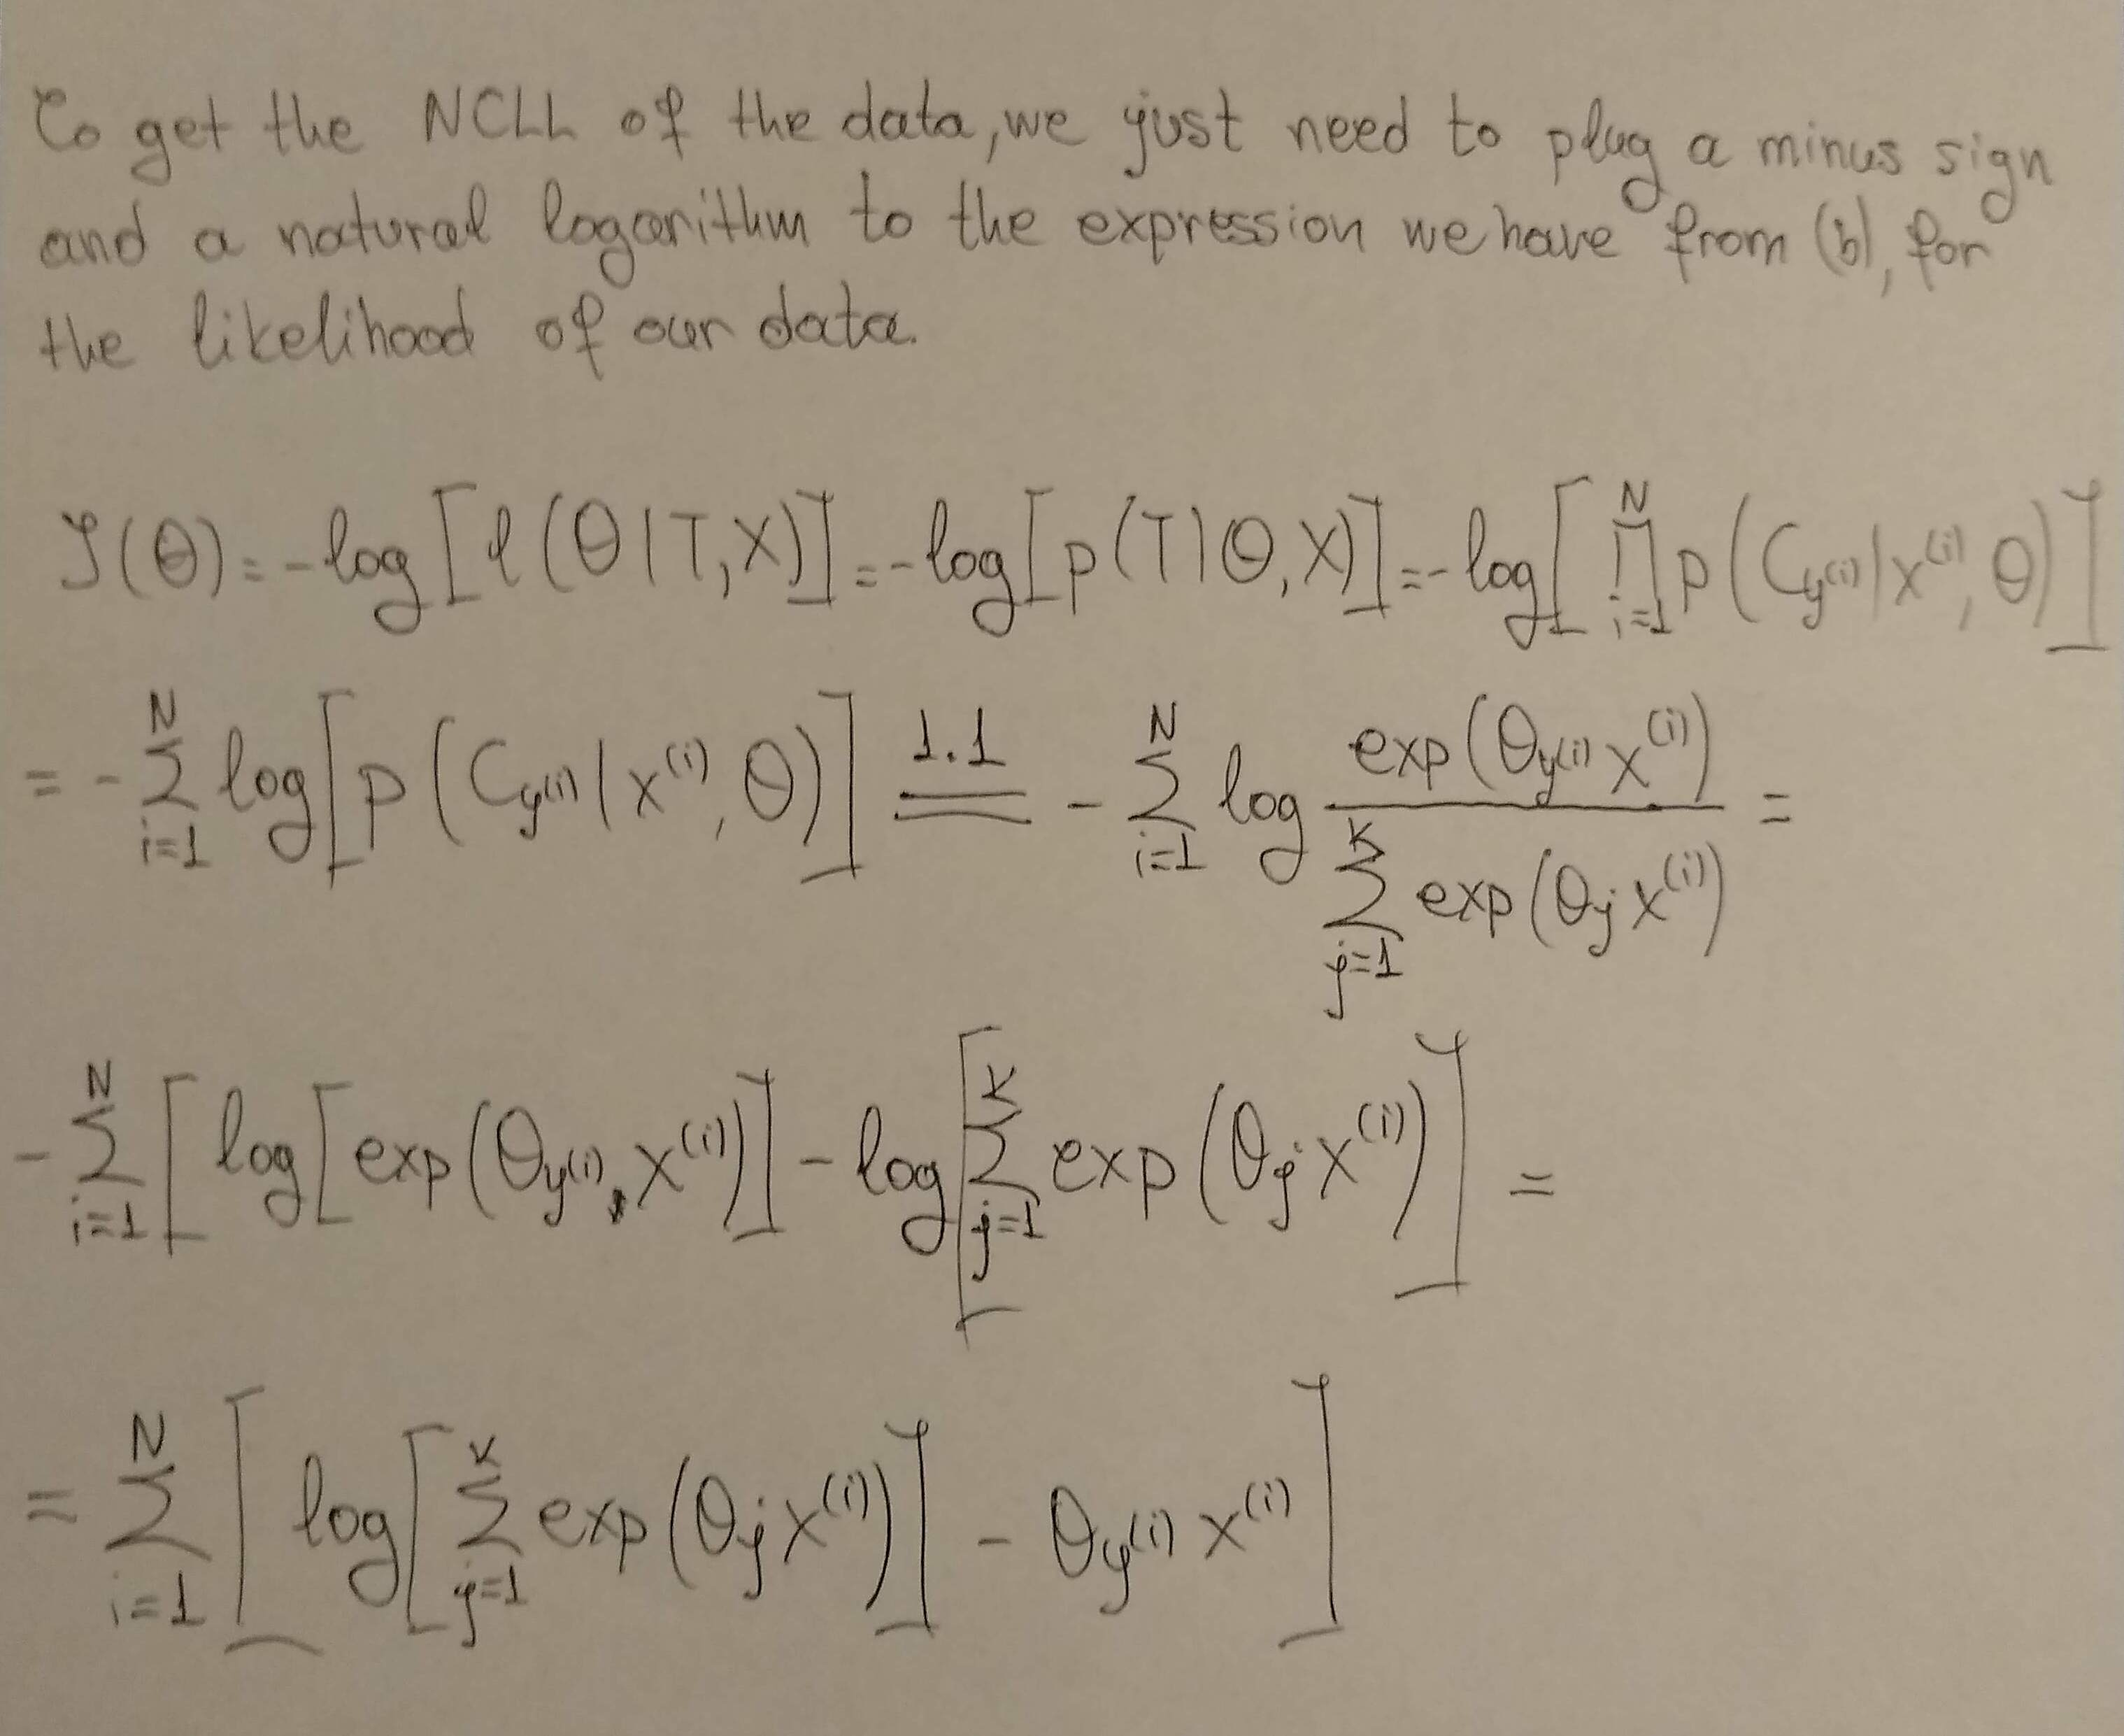
\includegraphics[scale=0.13]{pic2}
    \end{solution}
    
    \clearpage
    
    \item {\bf [4 points]} Now let's derive the partial derivative of the objective function with respect to the $k$th parameter vector $\thetav_k$. That is, derive $\frac{ \partial J(\Thetav) }{ \partial \thetav_k}$, where $J(\Thetav)$ is the objective function that you provided above. Show that the partial derivative  is as follows:

    $$
    \frac{\partial J(\Thetav)}{\partial \thetav_k} = - \sum_{i = 1}^N \left(\Tv_{i, k} - p\left(C_k \mid \xv^{(i)}, \Thetav\right)\right)  \xv^{(i)}
    $$
    
    Show all steps of the derivation. (\textbf{Hint:} A good first step would be to simplify your answer from part (c) as much as you can, if you haven't already done so in the previous part)
    
    
    \begin{solution}
    % If you are using the latex template, remove the empty spaces
    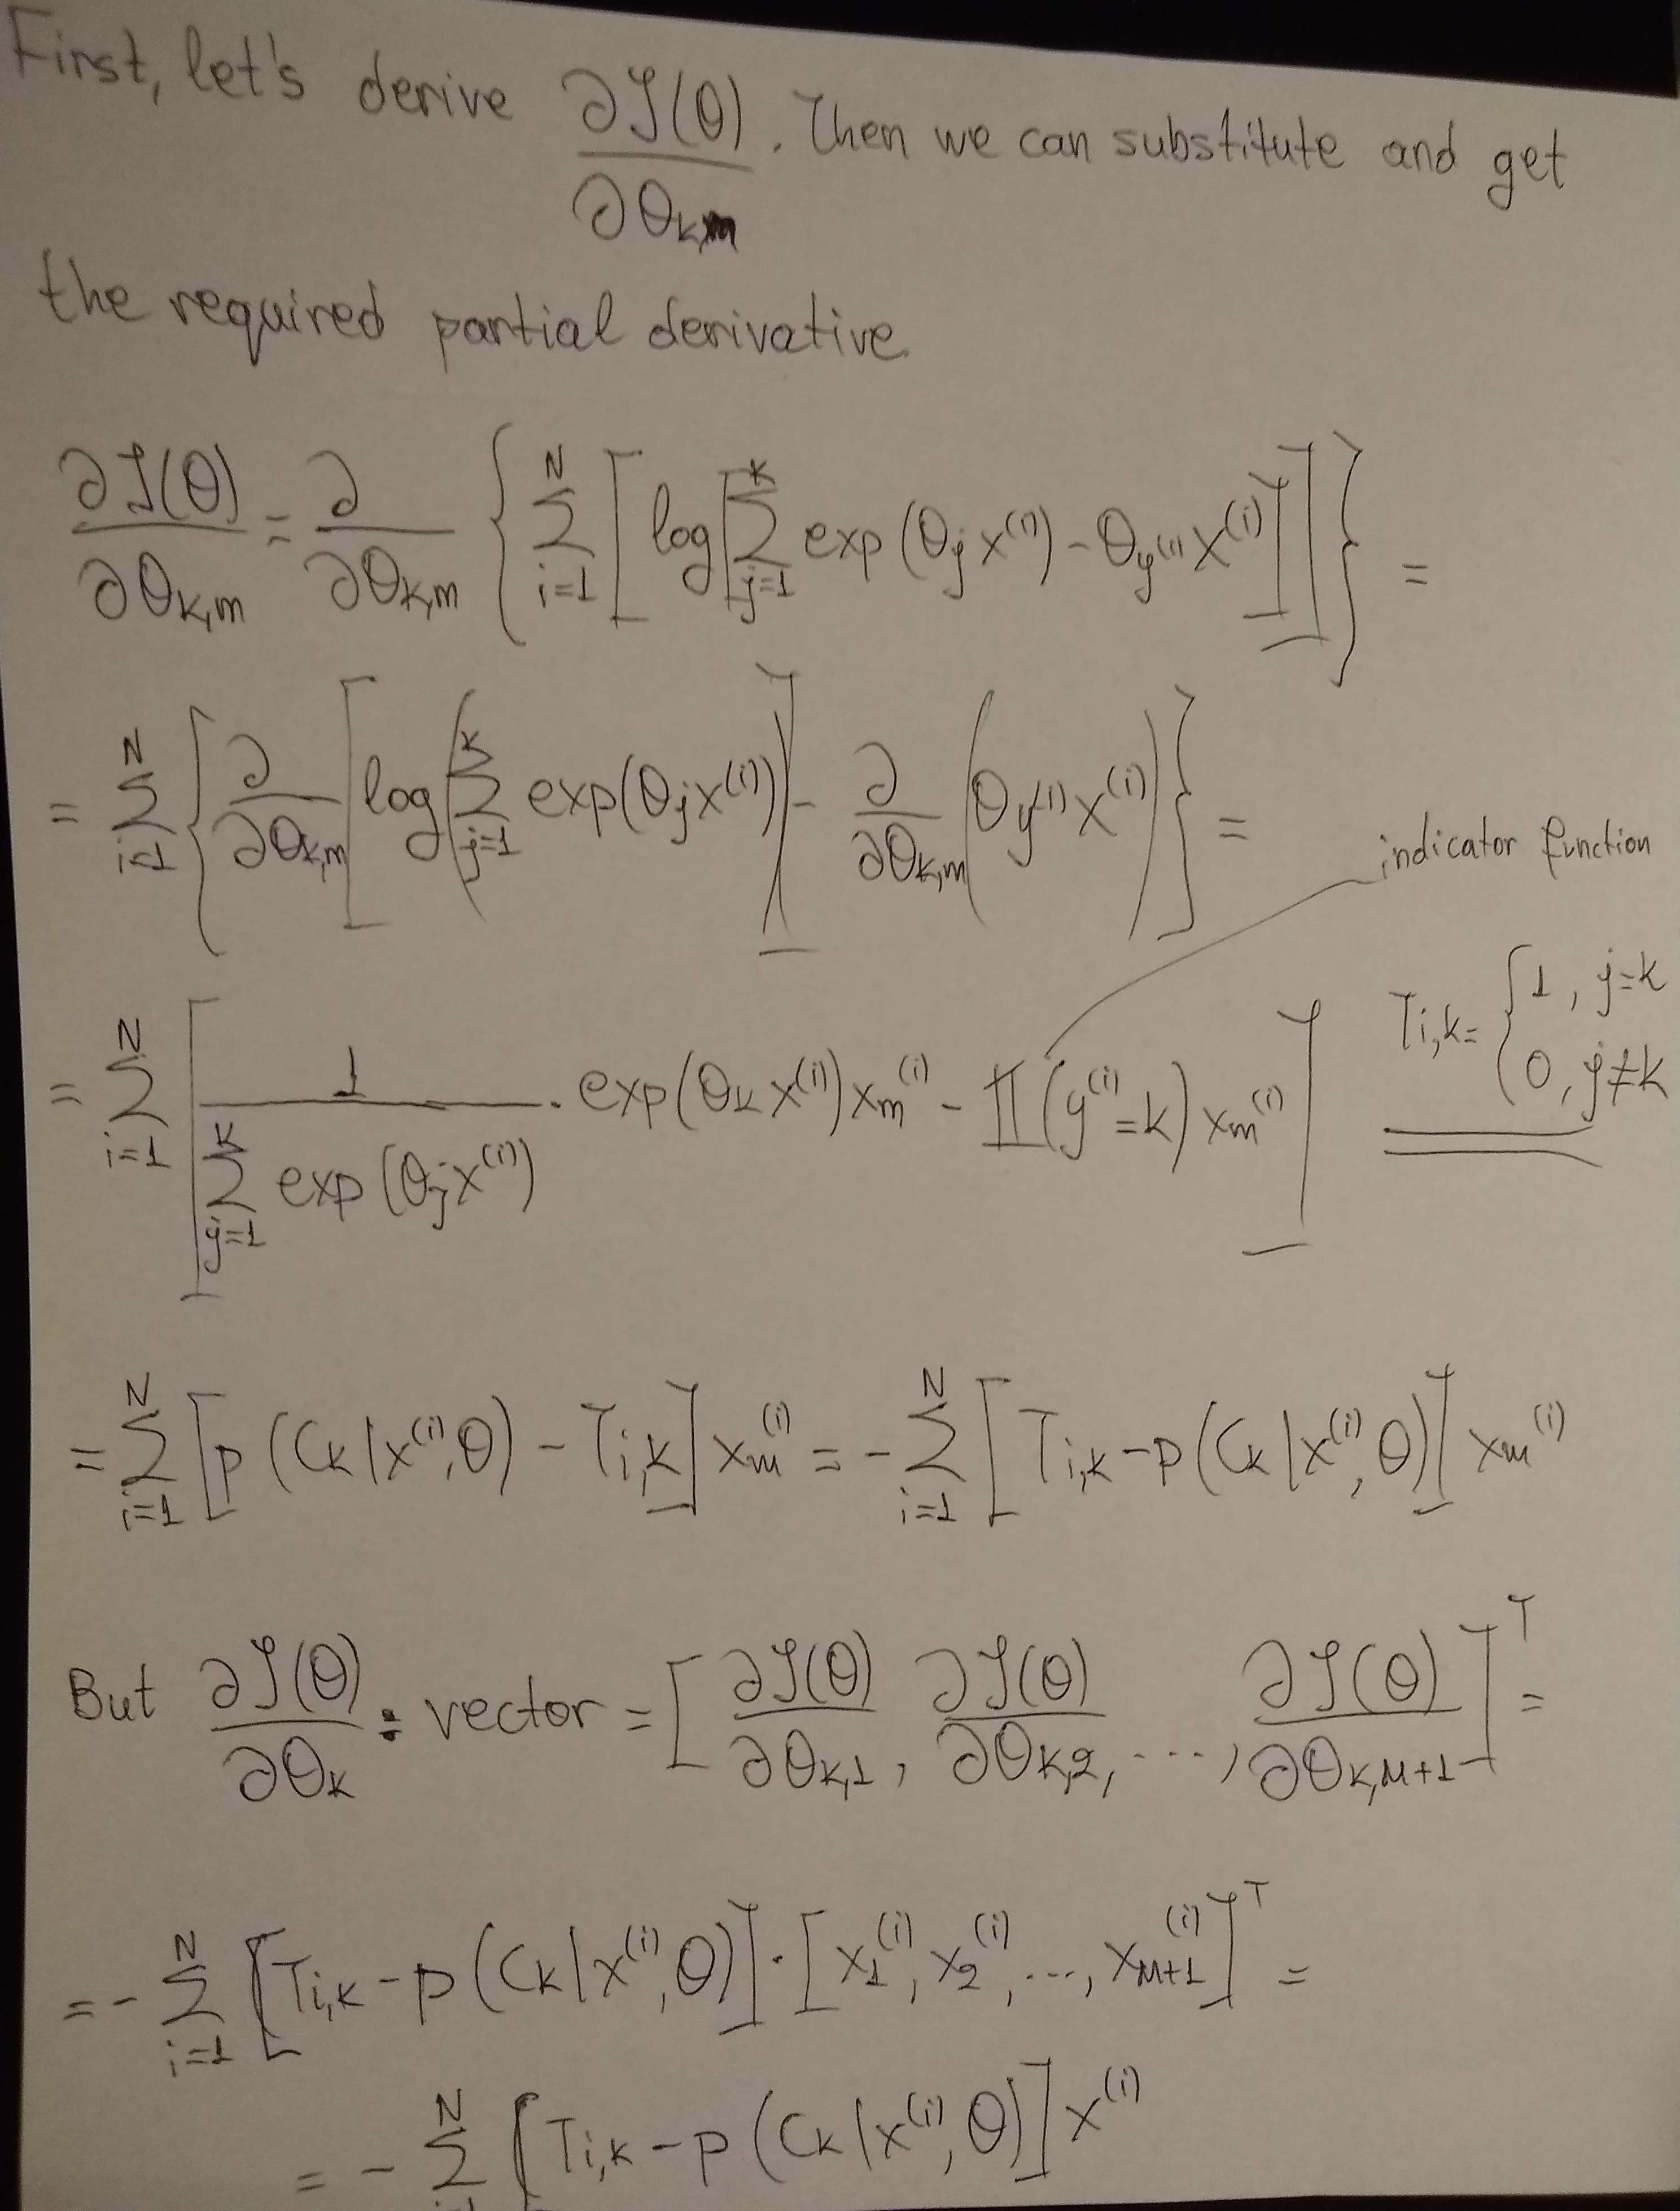
\includegraphics[scale=0.13]{pic3}
    \end{solution}
    
    \clearpage
    
    \item {\bf [2 points]} Write down the stochastic gradient descent update steps for an arbitrary $\theta_k$ using the $i^{th}$ training example in terms of $\mathbf{x^{(i)}}$, $\Tv_{i, k}$ and $p\left(C_k \mid \xv^{(i)}, \Thetav\right)$. 
    
    \textbf{Hint:} Recall the buggy SGD program from lecture.
    
    \begin{solution}
    % If you are using the latex template, remove the empty spaces
    
\includegraphics[scale=0.14]{pic4}
    
    \end{solution}
    
  
    \item {\bf [1 point]} If you train mutinomial logistic regression for infinite iterations without $\ell_1 = ||\Thetav||_1$ (sum of absolute values of all entries in the matrix ) or $\ell_2=||\Thetav||_2$ (square root of sum of squares of all entries in the matrix) regularization, the weights can go to infinity in magnitude. What is an explanation for this phenomenon? (\textbf{Hint}: Think about what happens to the probabilities if we train an unregularized logistic regression, and the role of the weights when calculating such probabilities)
    
     \begin{solution}
    % If you are using the latex template, remove the empty spaces
    If we train a multinomial logistic regression model for infinite iterations without applying any regularization technique our model will keep trying to fit the data with increasing accuracy. This means that the weights of our model are going to infinity, we will have high variance and our model will overfit the data, capturing the noise instead of generalizing. Adding an L1 or L2 regularizer will help decrease the magnitude of our weights, since we will now be trying to minimize the objective function with the addition of the absolute values of the weights or the squares of the weights respectively. Thus, decreasing the values of the weights the model will become more simple and capable to generalize better to held-out data.
    \end{solution}
    
    \clearpage
         
    \item {\bf [2 points]} How does regularization such as $\ell_1$ and $\ell_2$ help correct the problem?
    
    \textbf{Select all that apply:}
    \begin{list}{}
        \item $\square$ $\ell_1$ regularization prevents weights from going to infinity by eliminating the weights equal to 0, thus only include non-zero weights.
        \item $\blacksquare$ $\ell_1$ regularization prevents weights from going to infinity by reducing some of the weights to 0, thus removing some features all together. 
        \item $\blacksquare$ $\ell_2$ regularization prevents weights from going to infinity by reducing the magnitude of the the weights to \textit{close} to 0 (thus not removing any feature). 
        \item $\blacksquare$ Regularization such as $\ell_1$ or $\ell_2$ has the effect of preventing weights from going to infinity by appropriately penalizing the magnitude of the parameter vector elements.
    \end{list}

    
    \clearpage
   
    
\end{enumerate}
 \subsection{Binary Logistic Regression on a Small Dataset [5 points]}
 \label{sec:warm-up}
 The following questions should be completed before you start the programming portion of this assignment. (Section \ref{programming}).
 
 The following dataset consists of 4 training examples, where $x_k^{(i)}$ denotes the $k^{th}$ dimension of the $i^{th}$ training example, and the corresponding label $y^{(i)}$. $k \in \{1, 2, 3, 4, 5\}$ and $i \in \{1, 2, 3, 4\}$

\begin{center}
\begin{tabular}{|c|c|c|c|c|c|c|}
\hline
$i$ & $x_{1}$ & $x_{2}$ & $x_{3}$ & $x_{4}$ & $x_{5}$ & $y^{(i)}$ \\ \hline
1 & 0 & 0 & 1 & 0 & 1 & 0   \\ \hline
2 & 0 & 1 & 0 & 0 & 0 & 1     \\ \hline
3 & 0 & 1 & 1 & 0 & 0 & 1    \\ \hline
4 & 1 & 0 & 0 & 1 & 0 & 0   \\ \hline

\end{tabular}
\end{center}

A binary logistic regression model is trained on this data. After $n$ iterations, the parameter vector $\theta$ = $\lbrack 1.5, 2, 1, 2, 3 \rbrack^T$

Use the data above to answer the following questions. 
 \begin{enumerate}
     \item {\bf  [1 point] Negative log-likelihood} Calculate J($\theta$), the negative log-likelihood over the given data after iteration $n$. 
     \begin{solution}
    % If you are using the latex template, remove the empty spaces
    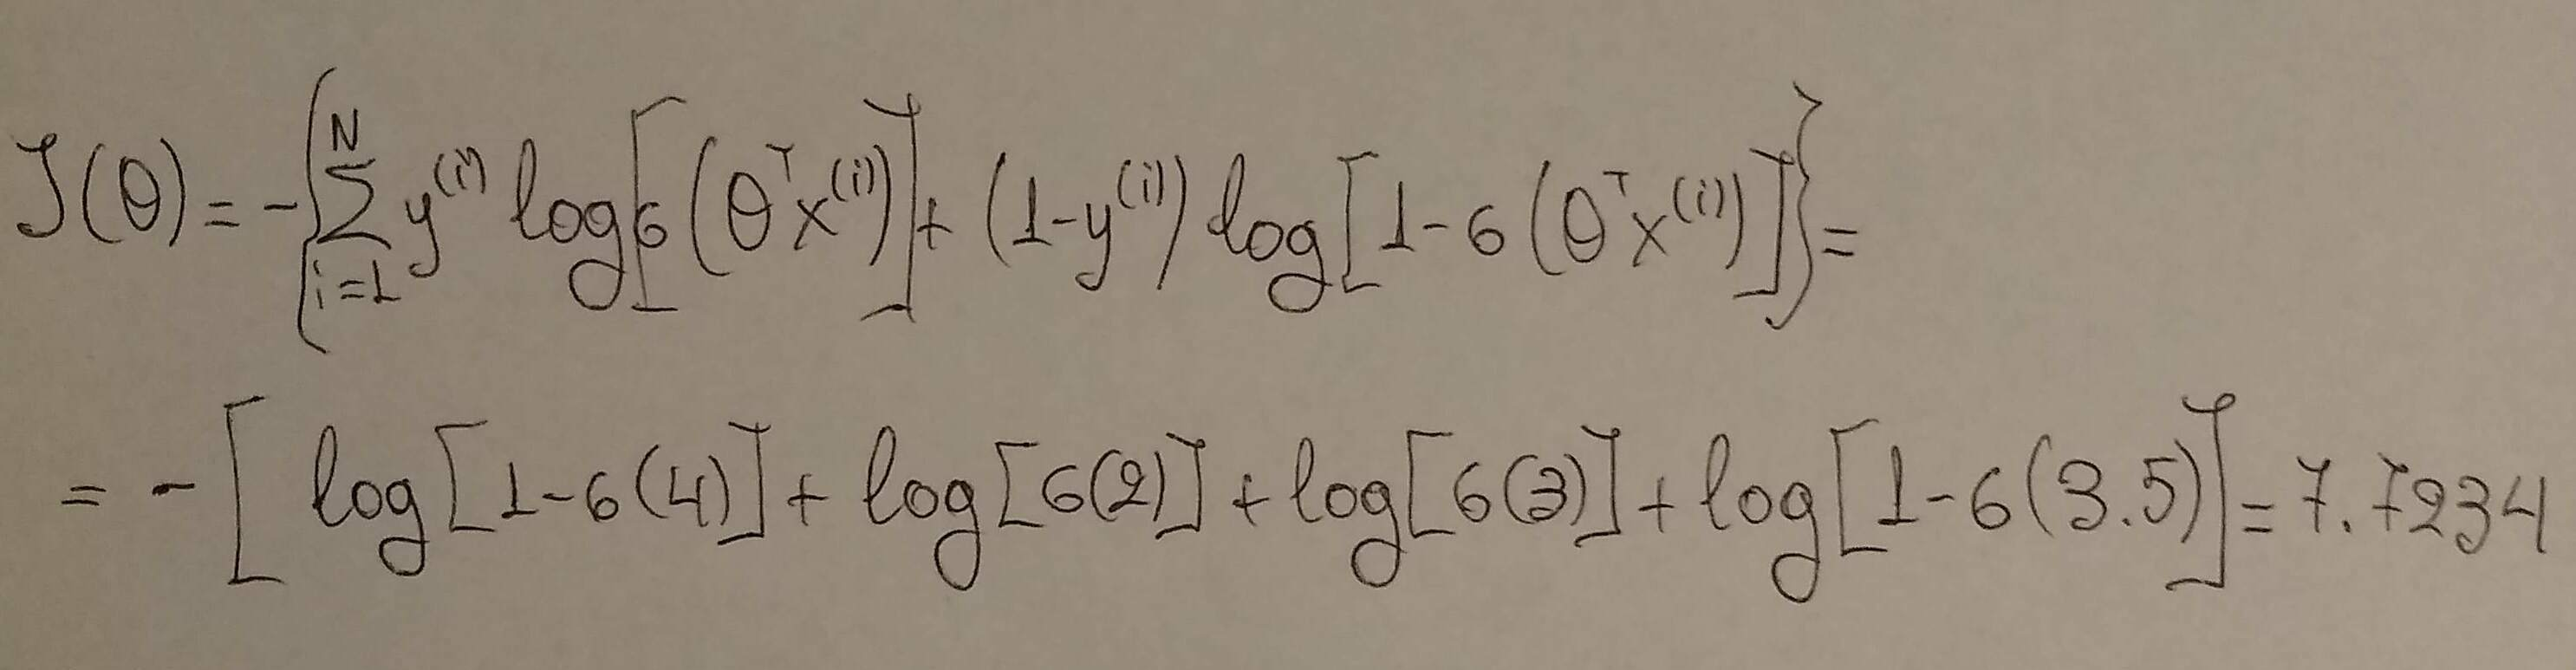
\includegraphics[scale=0.14]{pic5}
    \end{solution}
    \clearpage
    
     \item {\bf [2 points] Gradients} Calculate the gradients $\frac{\partial J(\thetav)}{\partial \thetav_j}$ with respect to $\theta_{j}$, for all $j \in \{1, 2, 3, 4, 5\}$
      \begin{solution}
    % If you are using the latex template, remove the empty spaces
    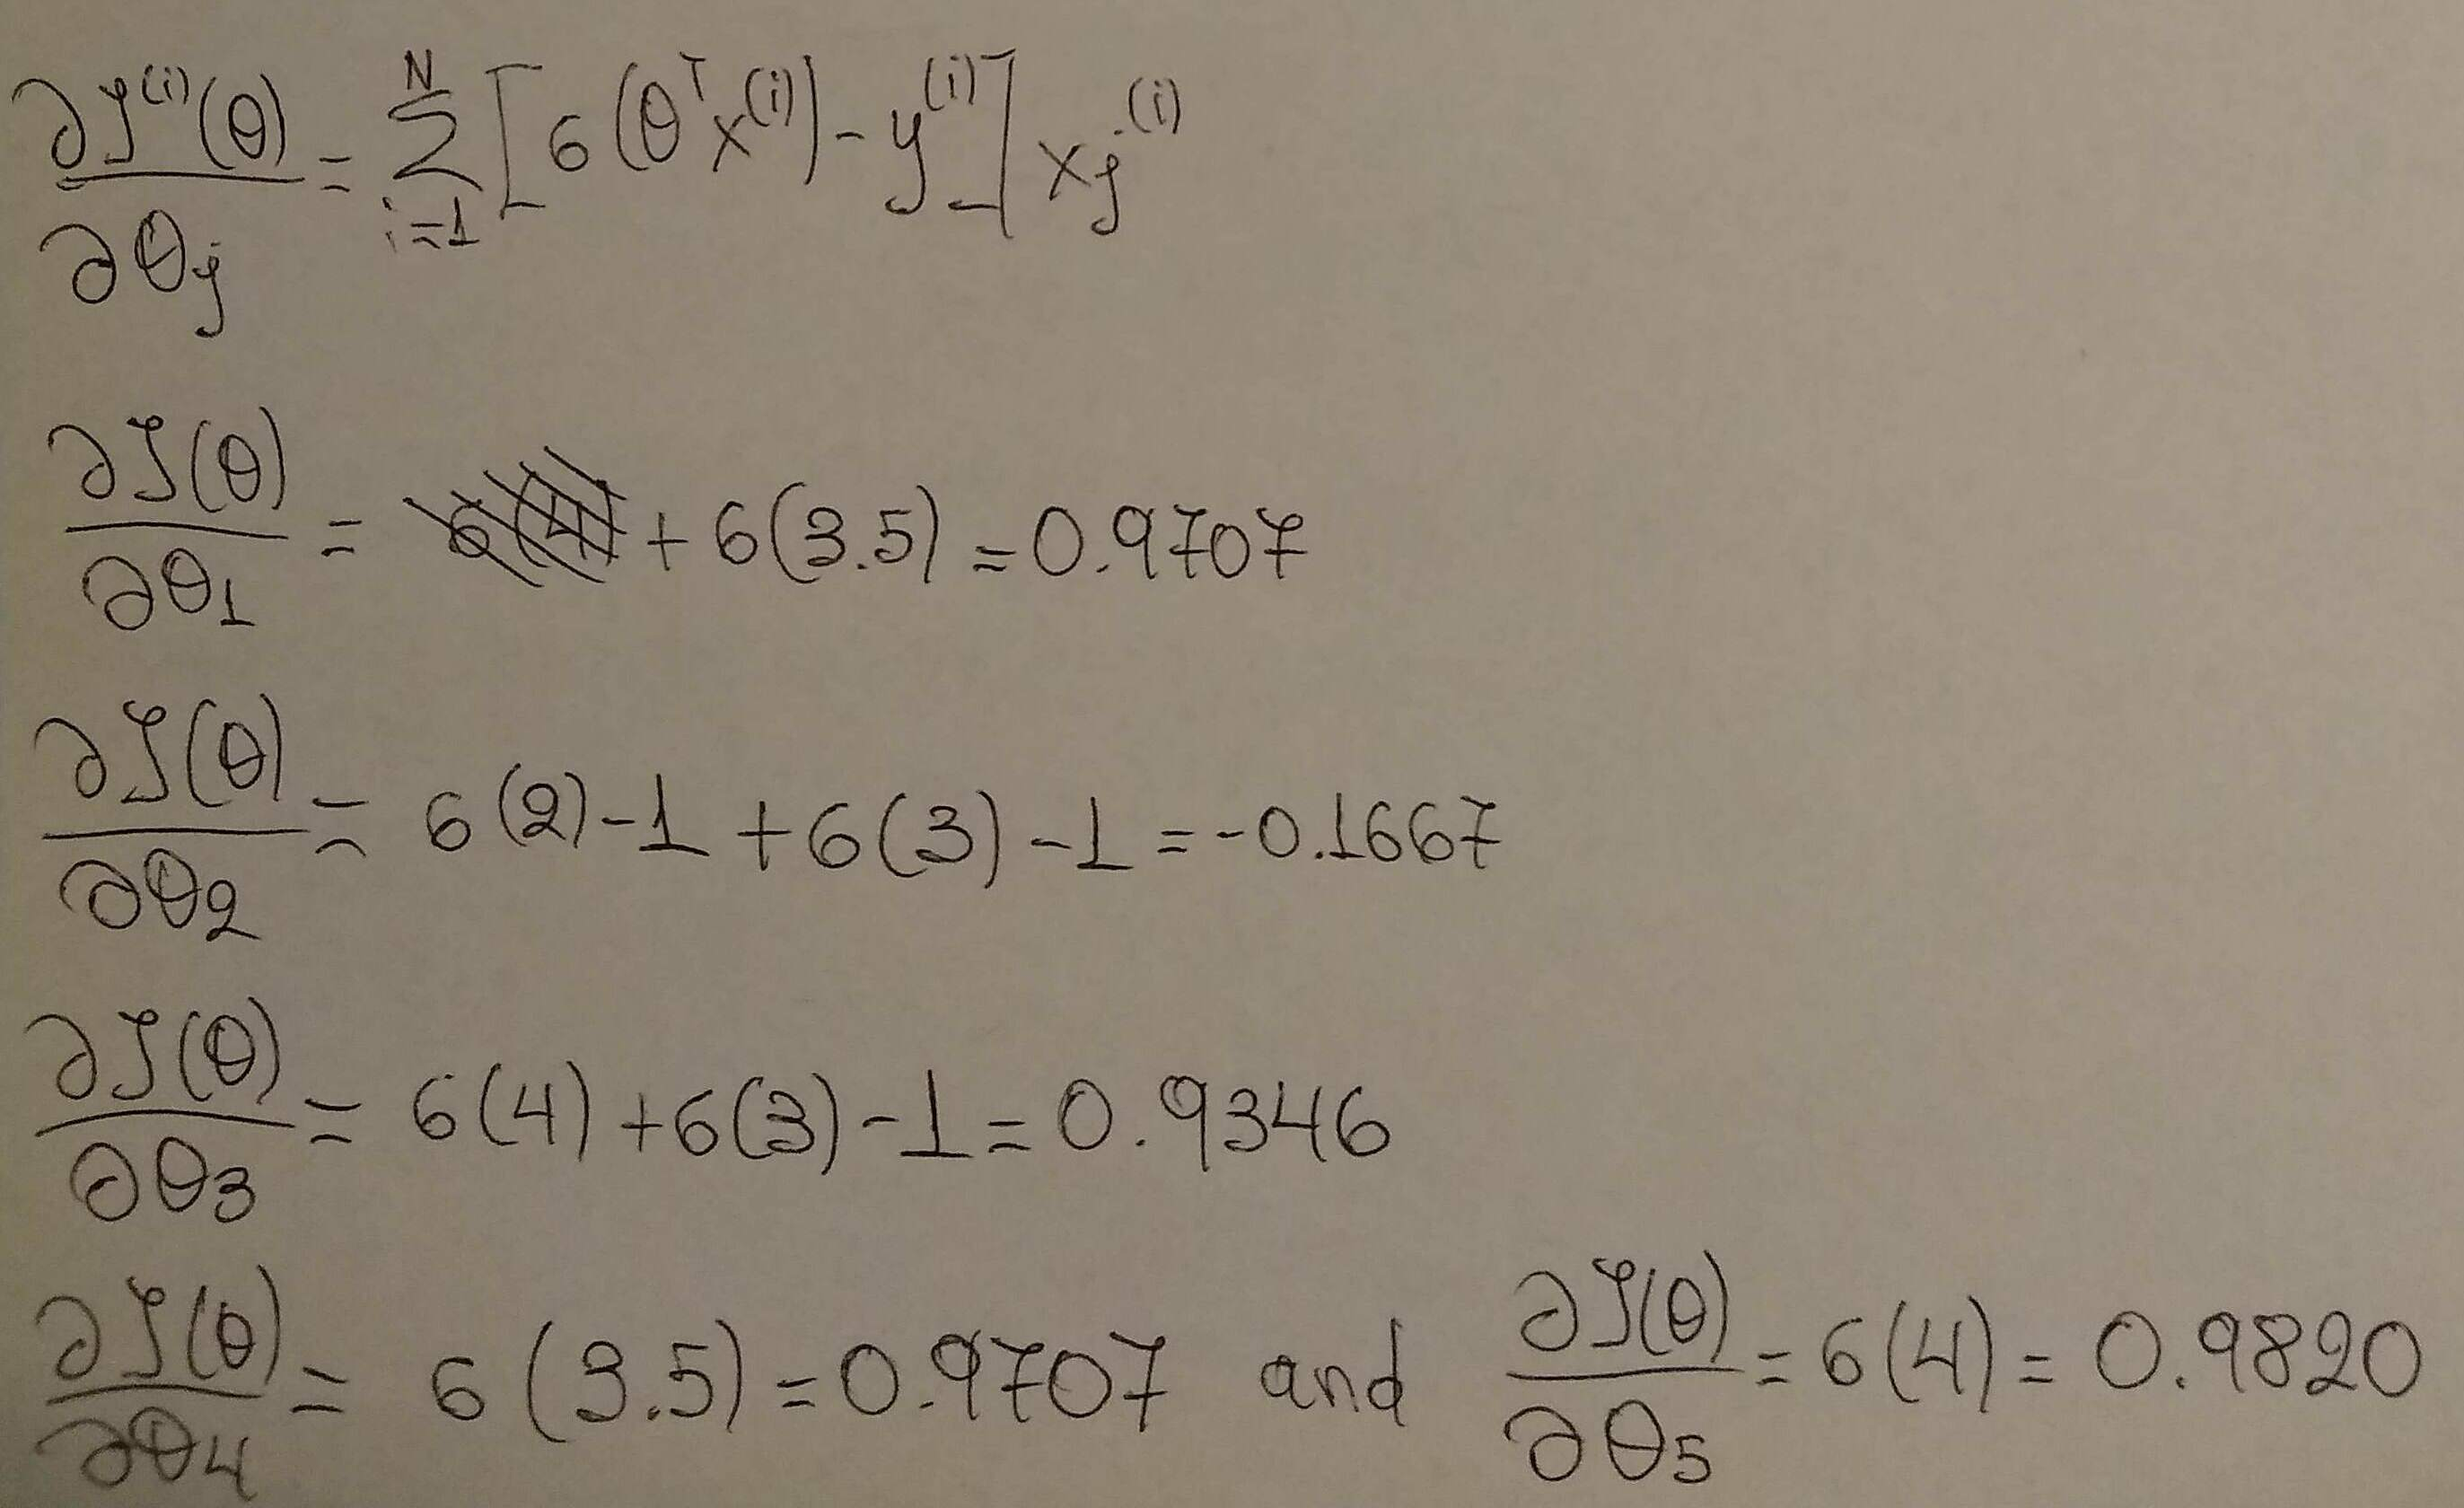
\includegraphics[scale=0.15]{pic6}
    \end{solution}
    
    
    \clearpage
     \item {\bf [1 point] Parameter Update} Update the parameters following the parameter update step $\thetav_j \leftarrow \thetav_j - \eta \frac{\partial J(\thetav)}{\partial \thetav_j}$ and give the final (numerical) value of the vector $\theta$. Consider $\eta$ = 1.
     \begin{solution}
    % If you are using the latex template, remove the empty spaces
    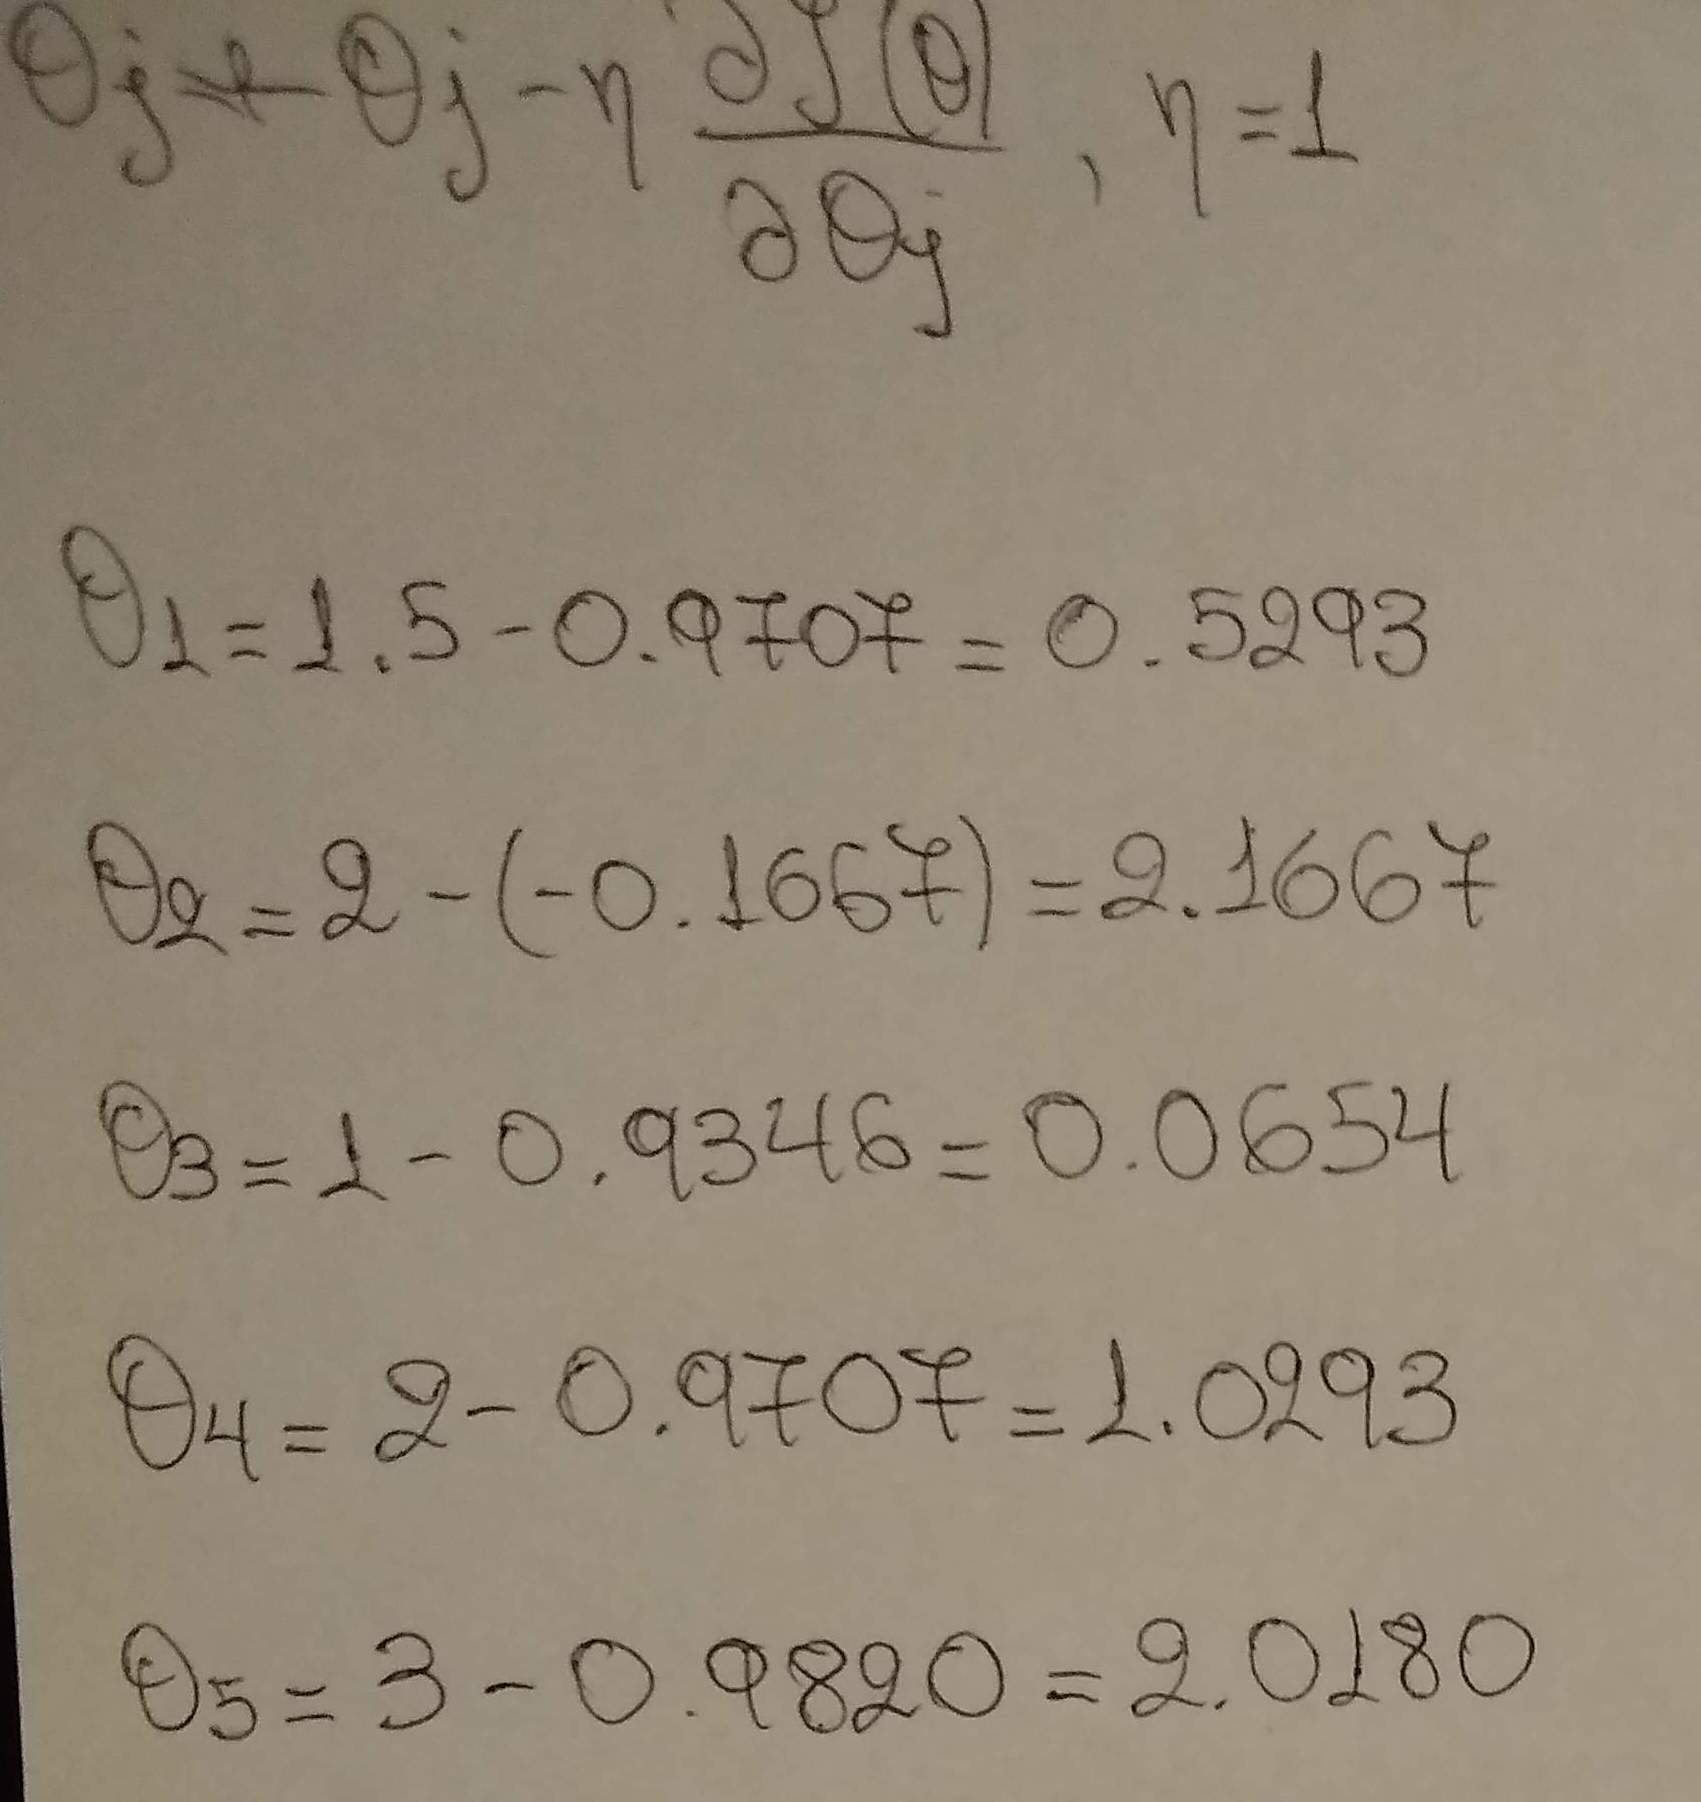
\includegraphics[scale=0.15]{pic7}
    \end{solution}
    
     \item {\bf  [1 point] Sparsity} Following table shows the sparse feature representation for the given data
     \begin{table}[h]
    \centering
     \begin{tabular}{cll}
    \toprule
    $i$ & {\bf label} $y^{(i)}$ & {\bf features} $\xv^{(i)}$ \\
    \midrule
    1 & 0 &  $\{ x_3: 1, x_5: 1 \}$ \\
    2 & 1 & $\{ x_2: 1 \}$ \\
    3 & 1 & $\{ x_2: 1, x_3: 1 \}$ \\
    4 & 0 & $\{ x_1: 1, x_4: 1 \}$ \\
    
    \bottomrule
    \end{tabular}
    \end{table}\\
    Calculate the probability $p\left(\y|\mathbf{X=x^{(3)}},\thetav\right)$ after the update step in 3., using \textbf{only k unique multiplication operations} where k is the number of non-zero features in $x_3$. Explicitly show these multiplication operations.
    \begin{solution}
    % If you are using the latex template, remove the empty spaces
    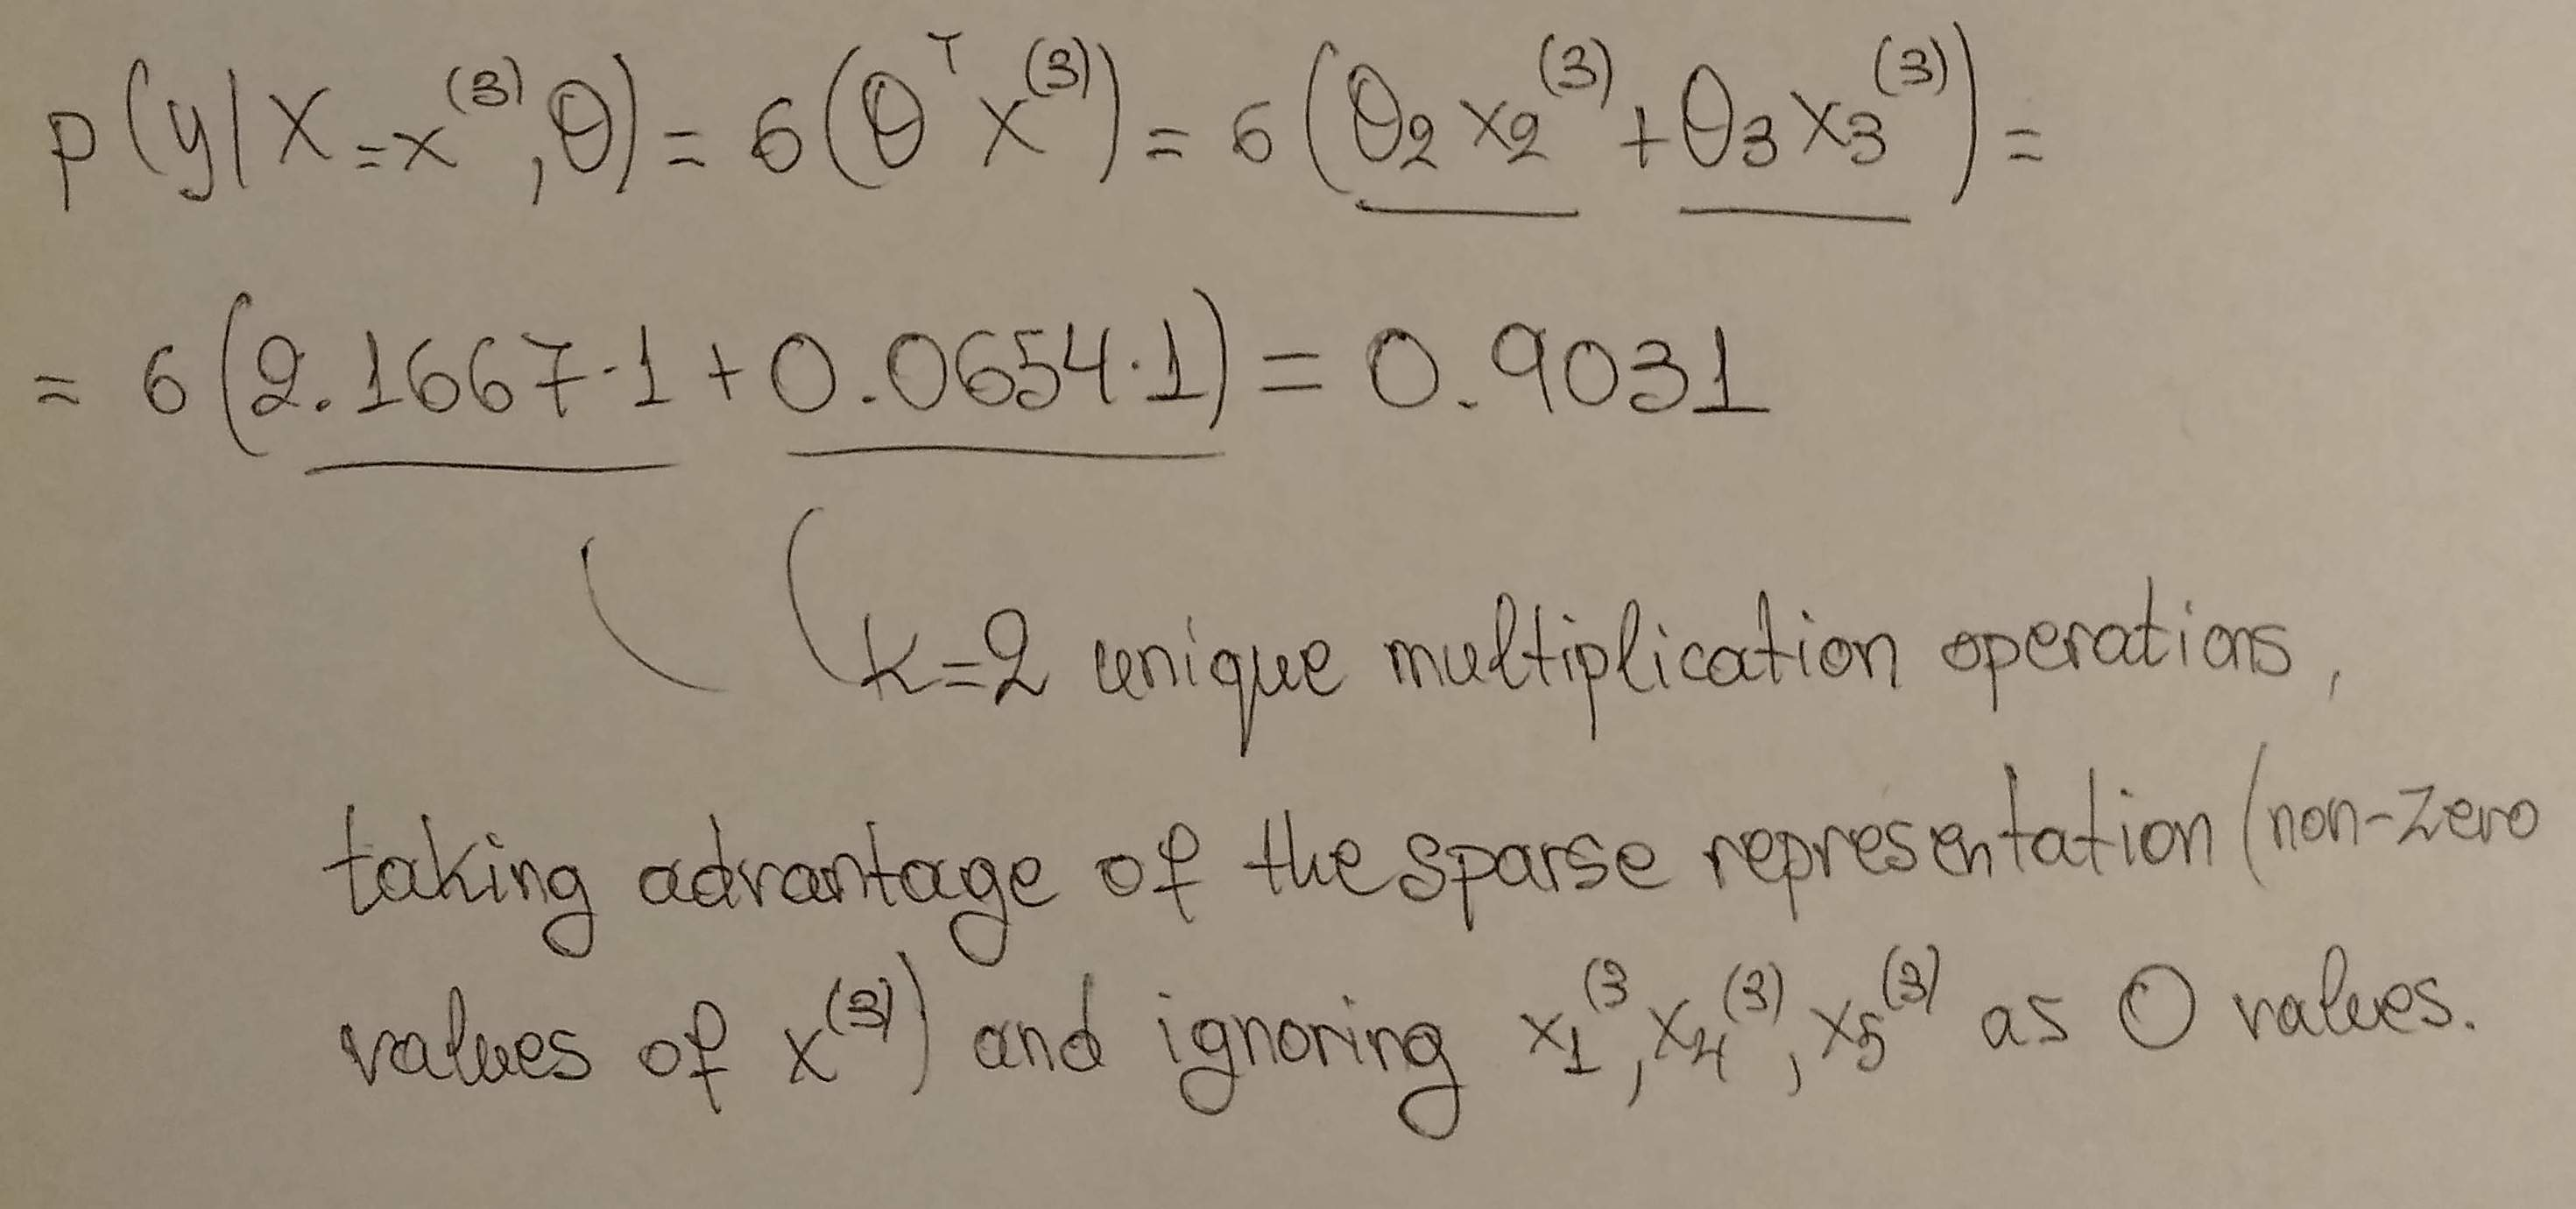
\includegraphics[scale=0.14]{pic8}
    \end{solution}
    

 \end{enumerate}
 \clearpage
\subsection{Programming Empirical Questions [8 points]}
\label{sec:empirical}

The following questions should be completed as you work through the programming portion of this assignment (Section \ref{programming}).

\begin{enumerate}
    
\item {\bf Plots [2 points]} 
For \emph{Model 1}, using the data in the largedata folder in the handout, make a plot that shows the \textit{average} negative log likelihood for the training and validation data sets after each of 200 epochs. The y-axis should show the negative log likelihood and the x-axis should show the number of epochs.  

\begin{solution}
    % If you are using the latex template, remove the empty spaces
    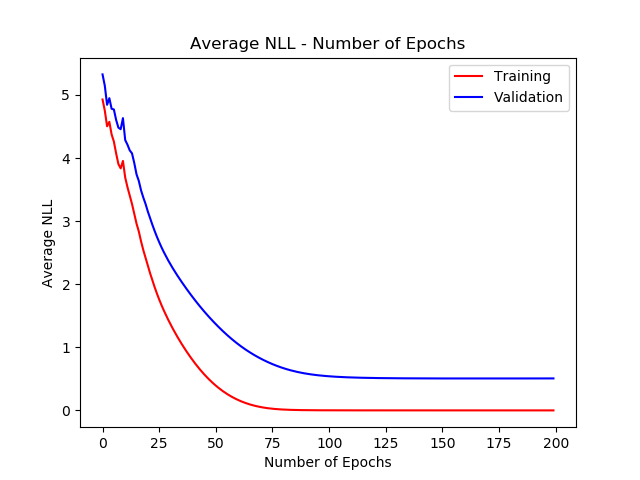
\includegraphics[scale=0.8]{model1}
\end{solution}

\item {\bf Plots [2 points]} 
For \emph{Model 2}, make a plot as in the previous question.
        
\begin{solution}
    % If you are using the latex template, remove the empty spaces
    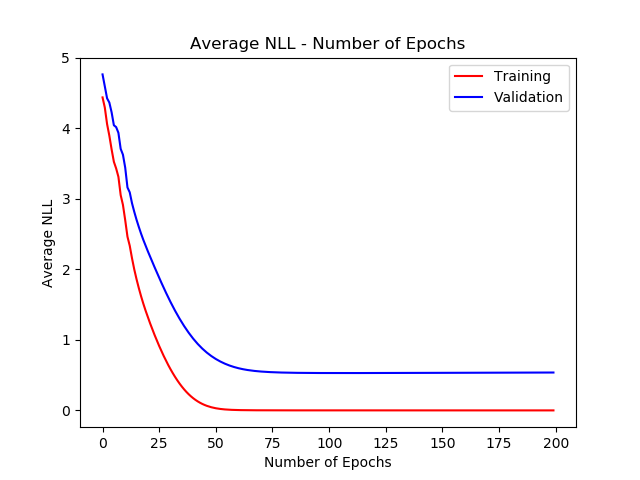
\includegraphics[scale=0.8]{model2}
\end{solution}
\clearpage


\item {\bf Explanation of Experiments [2 points]}
Write a few sentences explaining the output of the above experiments. In particular do the training and validation log likelihood curves look the same or different? Why?

\begin{solution}
    % If you are using the latex template, remove the empty spaces
    The curves for the training and validation values of the average negative log likelihood look similar for both model 1 and model 2. However, with careful observation we can notice that the model 2 curves are steeper and converge faster to a final loss function value. That is because the feature crafting we did for model 2, discarding words which appeared more than 3 times, improved our model and eventually performed better than the naive model 1, which considered every word that appeared in the training examples. Moreover, we can observe that for both models, the average NLL starts from approximately the same range of values for both the training and the validation data, but then, while our training curve keeps decreasing, at some point the validation curve decreases with a smaller rate and eventually "plateaus" at a larger value than the training error. This is what we expected, since the training error is low for our training dataset, but the validation error is higher, since it is considered as held-out data. It seems that our model can generalize well, since the validation curve looks close enough to the training curve.
\end{solution}

\item {\bf Results [2 points]} 
Make a table with your train and test error for the large data set (found in the largedata folder in the handout) for each of the 2 models after running for 50 epochs.

\begin{solution}
     \begin{table}[H]
        \centering
        \begin{tabular}{l|l|l}
        \toprule
        & Train Error & Test Error \\ 
        \midrule
        Model 1      &0.15         &0.32         \\ 
        Model 2 &0.01417         &0.1975         \\ 
        \bottomrule
        \end{tabular}
        \caption{``Large Data'' Results}
        \label{results}
    \end{table}
\end{solution}


        
\end{enumerate}

\newpage

\textbf{Collaboration Questions} Please answer the following:


    After you have completed all other components of this assignment, report your answers to the collaboration policy questions detailed in the Academic Integrity Policies found \href{http://www.cs.cmu.edu/~mgormley/courses/10601/about.html#7-academic-integrity-policies}{here}.
    \begin{enumerate}
        \item Did you receive any help whatsoever from anyone in solving this assignment? Is so, include full details.
        \item Did you give any help whatsoever to anyone in solving this assignment? Is so, include full details.
        \item Did you find or come across code that implements any part of this assignment ? If so, include full details.
    \end{enumerate}
    
    \begin{solution}
    % If you are using the latex template, remove the empty spaces
    1. No
    2. No
    3. No
    \end{solution}

\newpage

\section{Programming [70 points]}
\label{programming}

\subsection{The Task}\label{task}

Your goal in this assignment is to implement a working Natural Language Processing (NLP) system, i.e., a sentiment polarity analyzer, using binary logistic regression. You will then use your algorithm to determine whether a review is positive or negative using movie reviews as data. You will do some very basic feature engineering, through which you are able to improve the learner's performance on this task. You will write two programs: \texttt{feature.\{py|java|cpp|m\}} and \texttt{lr.\{py|java|cpp|m\}} to jointly complete the task. The programs you write will be automatically graded using the Autolab system. You may write your programs in {\bf Octave, Python, Java,} or {\bf C++}. However, you should use the same language for all parts below.

\textbf{Note}: Before starting the programming, you should work through section \ref{sec:warm-up} to get a good understanding of important concepts that are useful for this programming section. 

\subsection{The Datasets}\label{dataset}


  {\bf Datasets } Download the tar file from Autolab (``Download handout"). The tar file will contain all the data that you will need in order to complete this assignment. The handout contains data from the Movie Review Polarity dataset. \footnote{for more details, see \url{http://www.cs.cornell.edu/people/pabo/movie-review-data/}} In the data files, each line is a data point that consists of a label (0 for negatives and 1 for positives) and a attribute (a set of words as a whole). The label and attribute are separated by a tab.\footnote{The data files are in tab-separated-value (\lstinline{.tsv}) format. This is identical to a comma-separated-value (\lstinline{.csv}) format except that instead of separating columns with commas, we separate them with a tab character, \lstinline{\t}} In the attribute, words are separated using white-space (punctuations are also separated with white-space). All characters are lowercased. The format of each data point (each line) is \lstinline{label\tword1 word2 word3 ... wordN\n}.

Examples of the data are as follows:
 
\begin{lstlisting}
1 david spade has a snide , sarcastic sense of humor that works ... 
0 " mission to mars " is one of those annoying movies where , in ...
1 anyone who saw alan rickman's finely-realized performances in ...
1 ingredients : man with amnesia who wakes up wanted for murder , ...
1 ingredients : lost parrot trying to get home , friends synopsis : ... 
1 note : some may consider portions of the following text to be ...
0 aspiring broadway composer robert ( aaron williams ) secretly ...
0 america's favorite homicidal plaything takes a wicked wife in " ...
\end{lstlisting}

We have provided you with two subsets of the movie review dataset. Each dataset is divided into a training, a validation, and a test dataset.
%
The small dataset (\lstinline{smalltrain_data.tsv}, \lstinline{smallvalid_data.tsv}, and \lstinline{smalltest_data.tsv}) can be used while debugging your code. We have included the reference output files for this dataset after \textbf{30 training epochs} (see directory \lstinline{smalloutput/}). 
%
We have also included a larger dataset (\lstinline{train_data.tsv}, \lstinline{valid_data.tsv}, \lstinline{test_data.tsv}) with reference outputs for this dataset after \textbf{60 training epochs}  (see directory \lstinline{largeoutput/}) . This dataset can be used to ensure that your code runs fast enough to pass the autograder tests. Your code should be able to perform 60-epoch training and finish  predictions through all of the data in less than one minute for each of the models: one minute for Model 1 and one minute for Model 2.

  {\bf Dictionary } We also provide a dictionary file (\lstinline{dict.txt}) to limit the vocabulary to be considered in this assignment (this dictionary is constructed from the training data, so it includes all the words from the training data, but some words in validation and test data may not be present in the dictionary). Each line in the dictionary file is in the following format: \lstinline{word\tindex\n}. Words (column 1) and indexes (column 2) are separated with whitespace. Examples of the dictionary content are as follows: 
    \begin{lstlisting}
    films 0
    adapted 1
    from 2
    comic 3
    \end{lstlisting}
 
\subsection{Model Definition}\label{modeldescript}
 
 Assume you are given a dataset with $N$ training examples and $M$ features. We first write down the \emph{negative} conditional log-likelihood of the training data in terms of the design matrix $\Xv$, the labels $\yv$, and the parameter vector $\thetav$. This will be your objective function $J(\thetav)$ for gradient descent. 
%
(Recall that $i$th row of the design matrix $\Xv$ contains the features $\xv^{(i)}$ of the $i$th training example. The $i$th entry in the vector $\yv$ is the label $y^{(i)}$ of the $i$th training example.  Here we assume that each feature vector $\xv^{(i)}$ contains a bias \emph{feature}, e.g. $x_0^{(i)} = 1 \,\,\forall i \in \{1,\ldots,N\}$. As such, \textbf{the bias parameter is folded into our parameter vector $\thetav$.}


Taking $\x^{\left(i\right)}$ to be a $(M+1)$-dimensional vector where $x^{(i)}_0=1$, the likelihood $p\left(\y|\mathbf{X},\thetav\right)$ is:
\begin{align}
     p(\y |\mathbf{X},\thetav) &= \prod_{i = 1}^N p(y^{(i)} | \x^{(i)}, \thetav) = \prod_{i = 1}^N \left(\frac{e^{\thetav^T\x^{\left(i\right)}}}{1+e^{\thetav^T\x^{\left(i\right)}}}\right)^{y^{(i)}}\left(\frac{1}{1+e^{\thetav^T\x^{\left(i\right)}}}\right)^{\left(1-y^{(i)}\right)}\\
    &= \prod_{i=1}^N \frac{\left(e^{\thetav^T\x^{\left(i\right)}}\right)^{y^{(i)}}}{1+e^{\thetav^T\x^{\left(i\right)}}}
\end{align}
Hence, the negative conditional log-likelihood is:
\begin{align}
    J(\thetav)= -\log p\left(\y|\mathbf{X},\thetav\right) &= \sum_{i=1}^N  -y^{(i)}\left(\thetav^T\x^{\left(i\right)}\right)+\log\left(1+e^{\thetav^T\x^{\left(i\right)}}\right)
\end{align}


The partial derivative of the negative log-likelihood $J(\thetav)$ with respect to $\thetav_j \,, j\in\{0,...,M\}$ is:
\begin{align}
    \frac{\partial J(\thetav)}{\partial \thetav_j} &= -\sum_{i=1}^N \x_j^{\left(i\right)}\left[y^{(i)}-\frac{e^{\thetav^T\x^{\left(i\right)}}}{1+e^{\thetav^T\x^{\left(i\right)}}}\right]
\end{align}


The gradient descent update rule  for binary logistic regression for parameter element $\thetav_j$ is

\begin{align}
    \thetav_j \leftarrow \thetav_j - \eta \frac{\partial J(\thetav)}{\partial \thetav_j}
\end{align}


Then, the stochastic gradient descent update for  parameter element $\thetav_j$ using the $i$th datapoint $(\x^{(i)},y^{(i)})$ is:
\begin{align}
    \thetav_j \leftarrow \thetav_j + \eta \x_j^{\left(i\right)}\left[y^{(i)}-\frac{e^{\thetav^T\x^{\left(i\right)}}}{1+e^{\thetav^T\x^{\left(i\right)}}}\right]
\end{align}
 


\subsection{Implementation}

\subsubsection{Overview}\label{overview}

The implementation consists of two programs, a feature extraction program (\texttt{feature.\{py|java|cpp|m\}}) and a sentiment analyzer program (\texttt{lr.\{py|java|cpp|m\}}) using binary logistic regression. The programming pipeline is illustrated as follows.

\begin{figure}[H]
        \centering
        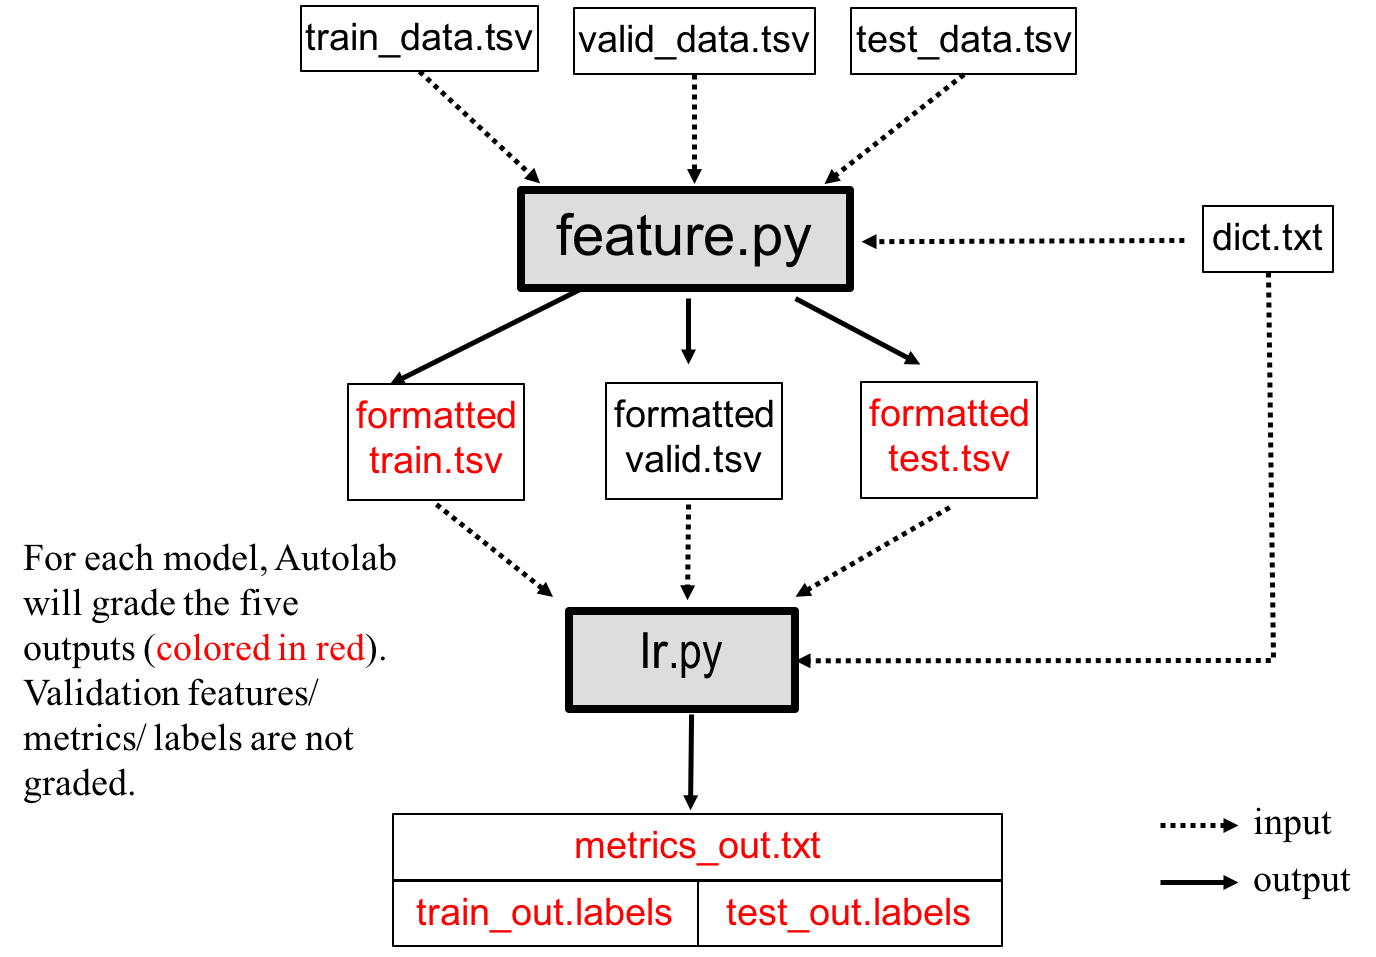
\includegraphics[width = 0.7\textwidth]{Pipeline.png}
        \caption{Programming pipeline for sentiment analyzer based on binary logistic regression}
        \label{pipeline}
\end{figure}


This first program is \texttt{feature.\{py|java|cpp|m\}}, that converts raw data (e.g., \lstinline{train_data.tsv}, \lstinline{valid_data.tsv}, and \lstinline{test_data.tsv}) into formatted training, validation and test data based on the vocabulary information in the dictionary file \lstinline{dict.txt}. To be specific, this program is to transfer the whole movie review text into a feature vector using some feature extraction methods. The formatted datasets should be stored in .tsv format. Details of formatted datasets will be introduced in Section~\ref{feature} and Section~\ref{format_output}.

The second program is \texttt{lr.\{py|java|cpp|m\}}, that implements a sentiment polarity analyzer using binary logistic regression. The file should learn the parameters of a binary logistic regression model that predicts a sentiment polarity (i.e. label) for the corresponding feature vector of each movie review. The program should output the labels of the training and test examples and calculate training and test error (percentage of incorrectly labeled reviews). As discussed in Appendix \ref{efficientdp} and \ref{datastructuredp}, efficient computation can be obtained with the help of the indexing information in the dictionary file \lstinline{dict.txt}.

\subsubsection{Feature Engineering} \label{feature}

Your implementation of \texttt{feature.\{py|java|cpp|m\}} should have an input argument \texttt{<feature\_flag>} that specifies one of two types of feature extraction structures that should be used by the logistic regression model. The two structures are illustrated below as probabilities of the labels given the inputs.

\begin{description}
    \item[Model 1] $p(y^{(i)} \mid \bf{1}_{occur}( \x^{(i)},Vocab), \thetav)$: This model defines a probability distribution over the current label $y^{(i)}$ using the parameters $\thetav$ and a \emph{bag-of-word} feature vector $\bf{1}_{occur}( \x^{(i)},Vocab)$ indicating which word in vocabulary $\bf{Vocab}$ of the dictionary occurs at least once in the movie review example $\x^{(i)}$. The entry in the indicator vector associated  to the occurring word will set to one (otherwise, it is zero). This bag-of-word model should be used when \texttt{<feature\_flag>} is set to 1.
    
    \item[Model 2] $p(y^{(i)} \mid \bf{1}_{trim}(  \x^{(i)},Vocab,$ $t), \thetav)$: This model defines a probability distribution over the current label $y^{(i)}$ using the parameters $\thetav$ and a \emph{trimmed} bag-of-word feature vector $\bf{1}_{trim}( \x^{(i)},Vocab,$ $t)$ indicating  (1) which word in vocabulary $\bf{Vocab}$ of the dictionary occurs in the movie review example $\x^{(i)}$, AND (2) the \emph{count of the word} is LESS THAN ($<$) threshold $t$. The entry in the indicator vector associated  to the word that satisfies both conditions will set to one (otherwise, it is zero, including no shown and high-frequent words). This trimmed bag-of-word model should be used when \texttt{<feature\_flag>} is set to 2. In this assignment, use the constant trimming threshold $t=4$.
    
\end{description}

The motivation of Model 2 is that keywords that truly represent the sentiment may not occur too frequently, this trimming strategy can make the feature presentation cleaner by removing highly repetitive words that are useless and neutral, such "the", "a", "to", etc. You will observe whether this basic and heuristic strategy based on this intuition will bring in performance improvement.

Note that above $\bf{1}_{occur}$ and $\bf{1}_{trim}$ are described as a dense feature representation as showed in Tables \ref{tab:model1dense} for illustration purpose. In your implementation, you should further convert it to the representation in \ref{tab:model1sparse} for Model 1 and the representation in \ref{tab:model2sparse} for Model 2, such that the formatted data outputs match Section~\ref{format_output}.



\subsubsection{Command Line Arguments}
The autograder runs and evaluates the output from the files generated, using the following command (note \lstinline{feature} will be run before \lstinline{lr}):

\begin{tabbing}
For Python: \=\texttt{\$ \textbf{python} feature.\textbf{py} [args1\dots]}\\
\>\texttt{\$ \textbf{python} lr.\textbf{py} [args2\dots]}\\
For Java: \>\texttt{\$ \textbf{java} feature.\textbf{java} [args1\dots]}\\
\>\texttt{\$ \textbf{java} lr.\textbf{java} [args2\dots]}\\
For C++: \>\texttt{\$ \textbf{g++} feature.\textbf{cpp} ./a.out [args1\dots]}\\
\>\texttt{\$ \textbf{g++} lr.\textbf{cpp} ./a.out [args2\dots]}\\
For Octave: \>\texttt{\$ \textbf{octave} -qH feature.\textbf{m} [args1\dots]}\\
\>\texttt{\$ \textbf{octave} -qH lr.\textbf{m} [args2\dots]}
\end{tabbing}

Where above \texttt{[args1\dots]} is a placeholder for eight command-line arguments:\texttt{<train\_input>}\newline \texttt{<validation\_input> <test\_input> <dict\_input> <formatted\_train\_out> \newline <formatted\_validation\_out>  <formatted\_test\_out> <feature\_flag>}. These arguments are described in detail below:
\begin{enumerate}
    \item \texttt{<train\_input>}: path to the training input \texttt{.tsv} file (see Section~\ref{dataset})
    \item \texttt{<validation\_input>}: path to the validation input \texttt{.tsv} file (see Section~\ref{dataset})
    \item \texttt{<test\_input>}: path to the test input \texttt{.tsv} file (see Section~\ref{dataset})
    \item \texttt{<dict\_input>}: path to the dictionary input \texttt{.txt} file (see Section~\ref{dataset})
    \item \texttt{<formatted\_train\_out>}: path to output \texttt{.tsv} file to which the feature extractions on the \emph{training} data should be written (see Section~\ref{format_output})
    \item \texttt{<formatted\_validation\_out>}: path to output \texttt{.tsv} file to which the feature extractions on the \emph{validation} data should be written (see Section~\ref{format_output})
    \item \texttt{<formatted\_test\_out>}: path to output \texttt{.tsv} file to which the feature extractions on the \emph{test} data should be written (see Section~\ref{format_output})
    \item \texttt{<feature\_flag>}: integer taking value 1 or 2 that specifies whether to construct the Model 1 feature set or the Model 2 feature set (see Section~\ref{feature})---that is, if \lstinline{feature_flag}==1 use Model 1 features; if \lstinline{feature_flag}==2 use Model 2 features
\end{enumerate}


On the other hand, \texttt{[args2\dots]} is a placeholder for eight command-line arguments:\texttt{<formatted\_train\_input>}\newline \texttt{<formatted\_validation\_input> <formatted\_test\_input> <dict\_input> <train\_out> \newline <test\_out> <metrics\_out> <num\_epoch>}. These arguments are described in detail below:
\begin{enumerate}
    \item \texttt{<formatted\_train\_input>}: path to the formatted training input \texttt{.tsv} file (see Section~\ref{format_output})
    \item \texttt{<formatted\_validation\_input>}: path to the formatted validation input \texttt{.tsv} file (see Section~\ref{format_output})
    \item \texttt{<formatted\_test\_input>}: path to the formatted test input \texttt{.tsv} file (see Section~\ref{format_output})
    \item \texttt{<dict\_input>}: path to the dictionary input \texttt{.txt} file (see Section~\ref{dataset})
    \item \texttt{<train\_out>}: path to output \texttt{.labels} file to which the prediction on the \emph{training} data should be written (see Section~\ref{output})
    \item \texttt{<test\_out>}: path to output \texttt{.labels} file to which the prediction on the \emph{test} data should be written (see Section~\ref{output})
    \item \texttt{<metrics\_out>}: path of the output \texttt{.txt} file to which metrics such as train and test error should be written (see Section~\ref{metrics})
    %\item \texttt{<model\_out>}: path of the output \texttt{.txt} file to which the model parameters should be written (see Section~\ref{model})
    \item \texttt{<num\_epoch>}: integer specifying the number of times SGD loops through all of the training data (e.g., if \texttt{<num\_epoch>} equals 5, then each training example will be used in SGD 5 times). 
\end{enumerate}

As an example, if you implemented your program in Python, the following two command lines would run your programs on the data provided in the handout for 60 epochs using the features from Model 1.

\begin{lstlisting}[language=Shell]
$ python feature.py train_data.tsv valid_data.tsv test_data.tsv \
dict.txt formatted_train.tsv formatted_valid.tsv formatted_test.tsv 1

$ python lr.py formatted_train.tsv formatted_valid.tsv formatted_test\
.tsv dict.txt train_out.labels test_out.labels metrics_out.txt 60

\end{lstlisting}

\begin{notebox}
{\bf Important Note:} You will not be writing out the predictions on validation data, only on train and test data. The validation data is \emph{only} used to give you an estimate of held-out negative log-likelihood at the end of each epoch during training. You are asked to graph the negative log-likelihood vs. epoch of the validation and training data in section \ref{sec:empirical}. \footnote{For this assignment, we will always specify the number of epochs. However, a more mature implementation would monitor the performance on validation data at the end of each epoch and stop SGD when this validation log-likelihood appears to have converged. You should \textbf{ \emph{not}} implement such a convergence check for this assignment.} 
\end{notebox}

\subsection{Program Outputs}

\subsubsection{Output: Formatted Data Files} \label{format_output}
Your \lstinline{feature} program should write three output \texttt{.tsv} files converting original data to formatted data on \texttt{<formatted\_train\_out>}, \texttt{<formatted\_valid\_out>}, and \texttt{<formatted\_test\_out>}. Each should contain the formatted presentation for each example printed on a new line. Use \lstinline{\n} to create a new line. The format for each line should exactly match 

label\lstinline{\t}index[word1]:value1\lstinline{\t}index[word2]:value2\lstinline{\t}...index[wordM]:valueM\lstinline{\n}

Where above, the first column is label, and the rest are "index[word]:value" feature elements. index[word] is the index of the word in the dictionary, and value is the value of this feature (in this assignment, the value is one or zero). There is a colon, \lstinline{:}, between index[word] and corresponding value. Columns are separated using a table character, \lstinline{\t}. The handout contains example \texttt{<formatted\_train\_out>}, \newline \texttt{<formatted\_valid\_out>}, and \texttt{<formatted\_test\_out>} for your reference.

The formatted output will be checked separately by the autograder by running your \lstinline{feature} program on some unseen datasets and evaluating your output file against the reference formatted files. Examples of content of formatted output file are given below.

\begin{lstlisting}
0	2915:1	21514:1	166:1	32:1	10699:1	305:1	...
0	7723:1	51:1	8701:1	74:1	370:1	8:1    ...
1	229:1	48:1	326:1	43:1	576:1	55:1	...
1	8126:1	1349:1	58:1	4709:1	48:1	8319:1	...
\end{lstlisting}


\subsubsection{Output: Labels Files} \label{output}
Your \lstinline{lr} program should produce two output \texttt{.labels} files containing the predictions of your model on training data (\texttt{<train\_out>}) and test data (\texttt{<test\_out>}). Each should contain the predicted labels for each example printed on a new line. Use \lstinline{\n} to create a new line. 

Your labels should exactly match those of a reference implementation -- this will be checked by the autograder by running your program and evaluating your output file against the reference solution. Examples of the content of the output file are given below.

\begin{lstlisting}
0
0
1
0
\end{lstlisting}

\subsubsection{Output Metrics} \label{metrics}
Generate a file where you report the following metrics: 

\begin{description}

\item[error] After the final epoch (i.e. when training has completed fully), report the final training error \newline \lstinline{error(train)} and test error \lstinline{error(test)}. 
\end{description}

All of your reported numbers should be within 0.01 of the reference solution. The following is the reference solution for large dataset with Model 1 feature structure after 60 training epochs. See \newline \lstinline{model1_metrics_out.txt} in the handout.

\begin{lstlisting}
error(train): 0.074167
error(test): 0.247500
\end{lstlisting}

Take care that your output has the exact same format as shown above. Each line should be terminated by a Unix line ending \lstinline{\n}. There is a whitespace character after the colon.

\subsection{Evaluation and Submission}

\subsubsection{Evaluation}

Autolab will test your implementations on hidden datasets with the same format as the two datasets provided in the handout. \lstinline{feature} program and \lstinline{lr} program will be tested separately. To ensure that your code can pass the autolab tests in under 5 minutes (the maximum time length) be sure that your code can complete 60-epoch training and finish predictions through all of the data in the \lstinline{largedata} folder in around one minute for each of the models.


\subsubsection{Requirements}
Your implementation must satisfy the following requirements:
\begin{itemize}
    \item The \texttt{feature.\{py|java|cpp|m\}} must produce a sparse representation of the data using the label-index-value format \{\lstinline{label index[word1]:value1  index[word2]:value2...\n} \}. We will use unseen data to test your feature output separately. (see Section~\ref{format_output} and Section~\ref{feature} on feature engineering for details on how to do this). 
    \item Ignore the words not in the vocabulary of \lstinline{dict.txt} when the analyzer encounters one in the test or validation data.
    \item Set the trimming threshold to a constant $t=4$ for Model 2 feature extraction (see Section~\ref{feature}). 
    \item Initialize all model parameters to $0$.
    \item Use stochastic gradient descent (SGD) to optimize the parameters for a binary logistic regression model. The number of times SGD loops through all of the training data (\texttt{num\_epoch}) will be specified as a command line flag. Set your learning rate as a constant  $\eta = 0.1$.
    \item Perform stochastic gradient descent updates on the training data \textbf{in the order that the data is given in the input file}. Although you would typically shuffle training examples when using stochastic gradient descent, in order to autograde the assignment, we ask that you {\bf DO NOT} shuffle trials in this assignment.
    \item Be able to select which one of two feature extractions you will use in your logistic regression model using a command line flag (see Section~\ref{feature})
    \item Do not hard-code any aspects of the datasets into your code. We will autograde your programs on multiple (hidden) datasets that include different attributes and output labels.
\end{itemize}

\subsubsection{Hints}
Careful planning will help you to correctly and concisely implement your program. Here are a few \emph{hints} to get you started.
\begin{itemize}
    \item Work through section \ref{sec:warm-up}
    \item Write a function that takes a single SGD step on the $i$th training example. Such a function should take as input the model parameters, the learning rate, and the features and label for the $i$th training example. It should update the model parameters in place by taking one stochastic gradient step.
    \item Write a function that takes in a set of features, labels, and model parameters and then outputs the error (percentage of labels incorrectly predicted). You can also write a separate function that takes the same inputs and outputs the negative log-likelihood of the regression model.
    \item You can either treat the bias term as separate variable, or fold it into the parameter vector. In either case, make sure you update the bias term correctly.  
\end{itemize}

\subsubsection{Autolab Submission}

You must submit a .tar file named {\tt lr.tar} containing \texttt{feature.\{py|m|java|cpp\}} and \newline \texttt{lr.\{py|m|java|cpp\}}.
You can create that file by running:
\begin{lstlisting}
tar -cvf lr.tar feature.{py|m|java|cpp} lr.{py|m|java|cpp}
\end{lstlisting}
from the directory containing your code. 

Some additional tips: {\bf DO NOT} compress your files; you are just
creating a tarball. Do not use tar \texttt{-czvf}.  {\bf DO NOT} put
the above files in a folder and then tar the folder.  Autolab is case
sensitive, so observe that all your files should be named in {\bf
  lowercase}. You must submit this file to the corresponding homework
link on Autolab. The autograder for Autolab prints out some additional 
information about the tests that it ran. You can view this output by selecting 
 "Handin History" from the menu and then clicking one of the scores you 
 received for a submission. For example on this assignment, among other things, 
 the autograder will print out which language it detects (e.g. Python, Octave, C++, Java).  {\bf It is recommended that you create a new empty folder somewhere else, copy your implementation files there, and create tarball from there. This can ensure a clean submission without tarring unnecessary files.}
 
 \begin{notebox}
  {\bf Python3 Users:} Please include a blank file called python3.txt (case-sensitive) in your tar submission and we will execute your submitted program using Python 3 instead of Python 2.7.
 \end{notebox}

Note: For this assignment, you may make up to 10 submissions to Autolab before the deadline, but only your last submission will be graded.
    
    
%%%%%%%%%%%%%%%%%%%%%%%%%%%%%%%%%%%%%%%%%%%%%%%%%%%%%%%%%%%%%%%%%%%%%%%%%%%%%%%%%%%


\newpage

\appendix
% TODO: Discussion of sparse gradient update
% TODO: Numerically stable softmax


\section{Implementation Details for Logistic Regression}

\subsection{Examples of Features}

Here we provide examples of the features constructed by Model 1 and Model 2. Table \ref{tab:inputfile} shows an example input file, where column $i$  indexes the $i$th movie review example. Rather than working directly with this input file, you should transform from the sentiment/text representation into a label/feature vector representation.

Table \ref{tab:model1dense} shows the dense occurrence-indicator representation expected for Model 1. The size of each feature vector (i.e. number of feature columns in the table) is equal to the size of the entire vocabulary of words stored in the given \lstinline{dict.txt} (this dictionary is actually constructed from the same training data in \lstinline{largeset}). Each row corresponds to a single example, which we have indexed by $i$.

It would be \emph{highly impractical} to actually store your feature vectors $\xv^{(i)} \in \Rb^M$ in the dense representation shown in Table \ref{tab:model1dense} which takes $O(M)$ space per vector ($M$ is around 40 thousands for the dictionary). This is because the features are extremely sparse: for the second example ($i=2$), only three of the features is non-zero for Model 1 and only two for Model 2. As such, we now consider a sparse representation of the features that will save both memory and computation.

Table \ref{tab:model1sparse} shows the sparse representation (bag-of-word representation) of the feature vectors. Each feature vector is now represented by a map from the index of the feature (e.g. {index[\tt "apple"]}) to its value which is 1. The space savings comes from the fact that we can omit from the map any feature whose value is zero. In this way, the map only contains \emph{non-zero entry} for each Model 1 feature vector.

Using the same sparse representation of features, we present an example of the features used by Model 2. This involves two step: (1) construct the count-of-word representation of the feature vector (see Table \ref{tab:countofword}); (2) trim/remove the highly repetitive words/features  and set the value of all remaining features to one (see Table \ref{tab:model2sparse}).




\subsection{Efficient Computation of the Dot-Product} \label{efficientdp}

In simple linear models like logistic regression, the computation is often dominated by the dot-product $\thetav^T \xv$ of the parameters $\thetav \in \Rb^M$ with the feature vector $\xv \in \Rb^M$ . When a dense representation of $\xv$ (such as that shown in Table \ref{tab:model1dense}) is used, this dot-product requires $O(M)$ computation. Why? Because the dot-product requires a sum over each entry in the vector:
\begin{align}
\thetav^T \xv = \sum_{m=1}^M \theta_m x_m
\end{align}
%
However, if our feature vector is represented sparsely, we can observe that the only elements of the feature vector that will contribute a non-zero value to the sum are those where $x_m \neq 0$, since this would allow $\theta_m x_m$ to be nonzero. As such, we can write the dot-product as below:
\begin{align}
\thetav^T \xv = \sum_{m \in \{1,\ldots,M\} \text{ s.t. } x_m \neq 0} \theta_m x_m
\label{eq:fastdot}
\end{align}
This requires only computation proportional to the number of non-zero entries in $\xv$, which is generally very small for Model 1 and Model 2 compared to the size of the vocabulary. To ensure that your code runs quickly it is best to write the dot-product in the latter form (Equation \eqref{eq:fastdot}).

\subsection{Data Structures for Fast Dot-Product} \label{datastructuredp}

Lastly, there is a question of how to implement this dot-product efficiently in practice. The key is choosing appropriate data structures. The most common approach is to choose a dense representation for $\thetav$. In C++ or Java, you could choose an array of \lstinline{float} or \lstinline{double}. In Python, you could choose a \lstinline{numpy} array or a list. 

To represent your feature vectors, you might need multiple data structures. First, you could create a shared mapping from a feature  name (e.g. {\tt apple} or {\tt boy}) to the corresponding index in the dense parameter vector. This shared mapping has already been provided to you in the \lstinline{dict.txt}, and you can extract the index of the word from the dictionary file for all later computation. In fact, you should be able to construct the dictionary on your own from the training data (we have done this step for you in the handout). Once you know the size of this mapping (which is the size of the dictionary file), you know the size of the parameter vector $\thetav$. 

Another data structure should be used to represent the feature vectors themselves. This assignment use the option to directly store a mapping from the integer index in the dictionary mapping (i.e. the index $m$) to the value of the feature $x_m$. Only the indexs of words satisfying certain conditions will be stored, and all other indexs are implies to have zero value of the feature $x_m$. This structure option will ensure that your code runs fast so long as you are doing an efficient computation instead of the $O(M)$ version.

\paragraph{Note for out-of-vocabulary features} The dictionary in the handout is made from the same training data in the large data set. You may encounter some words in the validation data and the test data that do not appear in the vocabulary mapping. In this assignment, you should ignore those words during prediction and evaluation.


\begin{table}[p]
    \centering
%
\begin{tabular}{cll}
\toprule
{\bf example index} $i$  & {\bf sentiment $y^{(i)}$ } & {\bf review text $\x^{(i)}$ }\\
\midrule
1 & pos & apple boy , cat dog \\
2 & pos & boy boy : dog dog ; dog dog . dog egg egg \\
3 & neg & apple apple apple apple boy cat cat dog \\
4 & neg & egg fish \\

\bottomrule
\end{tabular}
%
    \caption{Abstract representation of the input file format.  The $i$th row of this file will be used to construct the $i$th training example using either Model 1 features (Table \ref{tab:model1sparse}) or Model 2 features (Table \ref{tab:model2sparse}).}
    \label{tab:inputfile}
\end{table}


\begin{table}[p]
    \centering
%
\begin{tabular}{clllllllllllll}
\toprule
$i$ & {\bf label} $y^{(i)}$ & \multicolumn{12}{l}{ {\bf features} $\xv^{(i)}$  }\\
& & \rot{\tt zoo} & \rot{$\ldots$} & \rot{\tt apple} & \rot{\tt boy} & \rot{\tt cat} & \rot{\tt dog} & \rot{\tt egg} & \rot{\tt fish} & \rot{\tt girl} & \rot{\tt head} & \rot{$\ldots$} & \rot{\tt zero} \\
\midrule
1 & 1                    & 0 & $\ldots$ & 1 & 1 & 1 & 1 & 0 & 0 & 0 & 0 & $\ldots$ & 0 \\ 
2 & 1                    & 0 & $\ldots$ & 0 & 1 & 0 & 1 & 1 & 0 & 0 & 0 & $\ldots$ & 0 \\ 
3 & 0                    & 0 & $\ldots$ & 1 & 1 & 1 & 1 & 0 & 0 & 0 & 0 & $\ldots$ & 0 \\ 
4 & 0                    & 0 & $\ldots$ & 0 & 0 & 0 & 0 & 1 & 1 & 0 & 0 & $\ldots$ & 0 \\ 

\bottomrule
\end{tabular}
%
    \caption{Dense feature representation for Model 1 corresponding to the input file in Table \ref{tab:inputfile}. The $i$th row corresponds to the $i$th training example. Each dense feature has the size of the vocabulary in the dictionary. Punctuations are excluded.}
    \label{tab:model1dense}
\end{table}


\begin{table}[p]
    \centering
%
\begin{tabular}{cll}
\toprule
$i$ & {\bf label} $y^{(i)}$ & {\bf features} $\xv^{(i)}$ \\
\midrule
1 & 1 &  \{ index[``{\tt apple}'']: 1, index[``{\tt boy}'']: 1, index[``{\tt cat}'']: 1, index[``{\tt dog}'']: 1 \} \\
2 & 1 & \{ index[``{\tt boy}'']: 1, index[``{\tt dog}'']: 1, index[``{\tt egg}'']: 1 \} \\
3 & 0 & \{ index[``{\tt apple}'']: 1, index[``{\tt boy}'']: 1, index[``{\tt cat}'']: 1, index[``{\tt dog}'']:1 \} \\
4 & 0 & \{ index[``{\tt egg}'']: 1, index[``{\tt fish}'']: 1 \} \\

\bottomrule
\end{tabular}
%
    \caption{Sparse feature representation (bag-of-word representation) for Model 1 corresponding to the input file in Table \ref{tab:inputfile}.}
    \label{tab:model1sparse}
\end{table}




\begin{table}[p]
    \centering
%
\begin{tabular}{cll}
\toprule
$i$ & {\bf label} $y^{(i)}$ & {\bf features} $\xv^{(i)}$ \\
\midrule
1 & 1 &  \{ index[``{\tt apple}'']: 1, index[``{\tt boy}'']: 1, index[``{\tt cat}'']: 1, index[``{\tt dog}'']: 1 \} \\
2 & 1 & \{ index[``{\tt boy}'']: 2, index[``{\tt dog}'']: 5, index[``{\tt egg}'']: 2 \} \\
3 & 0 & \{ index[``{\tt apple}'']: 4, index[``{\tt boy}'']: 1, index[``{\tt cat}'']: 2, index[``{\tt dog}'']: 1 \} \\
4 & 0 & \{ index[``{\tt egg}'']: 1, index[``{\tt fish}'']: 1 \} \\
\bottomrule
\end{tabular}
%
    \caption{Count of word representation  for Model 2 corresponding to the input file in Table \ref{tab:inputfile}. }
    \label{tab:countofword}
\end{table}

\begin{table}[p]
    \centering
%
\begin{tabular}{cll}
\toprule
$i$ & {\bf label} $y^{(i)}$ & {\bf features} $\xv^{(i)}$ \\
\midrule
1 & 1 &  \{ index[``{\tt apple}'']: 1, index[``{\tt boy}'']: 1, index[``{\tt cat}'']: 1, index[``{\tt dog}'']: 1 \} \\
2 & 1 & \{ index[``{\tt boy}'']: 1,  index[``{\tt egg}'']:1 \} \\
3 & 0 & \{  index[``{\tt boy}'']: 1, index[``{\tt cat}'']: 1, index[``{\tt dog}'']: 1 \} \\
4 & 0 & \{ index[``{\tt egg}'']: 1, index[``{\tt fish}'']: 1 \} \\
\bottomrule
\end{tabular}
%
    \caption{Sparse feature representation for Model 2 corresponding to the input file in Table \ref{tab:inputfile}. Assume that the trimming threshold is 4. As a result, "dog" in example 2 and "apple" in example 3 are removed and the value of all remaining features are reset to value 1.}
    \label{tab:model2sparse}
\end{table}


%\bibliographystyle{abbrv}
%\bibliography{references}

\end{document}




